\chapter{The \proglang{R} Package \pkg{forestinventory}: design-based global and small area estimations for multi-phase forest inventories}
\label{chap:rpack}
{\large Andreas Hill$^1$, Alexander Massey$^1$}\\

\vspace{3cm}
\noindent
$^1$ETH Z\"urich\\Department of Environmental Systems Science,Universit\"atstrasse 16, 8092 Z\"urich, Switzerland \\

\vspace{\fill}
\noindent
Submitted to:\\
\textit{Journal of Statistical Software} (accepted subject to minor revisions).

\newpage
\thispagestyle{plain}
\renewcommand{\labelitemi}{--}
\begin{itemize}
	\item Alexander Massey is co-author of the R package \textit{forestinventory} and supported writing of the manuscript.
\end{itemize}

\clearpage
%%%%%%%%%%%%%%
%% Abstract %%
%%%%%%%%%%%%%%
\section*{Abstract}
\label{chap:rpack:Abstract}
Forest inventories provide reliable evidence-based information to assess the state and development of forests over time.  They typically consist of a random sample of plot locations in the forest that are assessed individually by hand. Due to the high costs of these terrestrial campaigns, remote sensing information available in high quantity and low costs is frequently incorporated in the estimation process in order to reduce inventory costs or improve estimation precision. With respect to this objective, the application of multi-phase forest inventory methods (e.g., double- and triple-sampling regression estimators) has proved to be efficient. While these methods have been successfully applied in practice, the availability of open-source software has been rare if not non-existent. The \proglang{R} package \pkg{forestinventory} provides a comprehensive set of global and small area regression estimators for multi-phase forest inventories under simple and cluster sampling. The implemented methods have been demonstrated in various scientific studies ranging from small to large scale forest inventories, and can be used for post-stratification, regression and regression within strata. This article summarizes the mathematical theory of this family of design-based estimators and demonstrates their application in the \proglang{R} environment.


%------------------------------------------------------------------------------------------------%
% ---------------------------------- Introduction ---------------------------------------------- %

\section{Introduction}
\label{sec:intro}


In many countries, forest inventories have become an indispensable tool for evaluating the current state of forests as well as for tracking their development over time. They provide accurate quantitative information that can be used to define management actions and to adapt forest management strategies according to guidelines on national and international levels. As conducting a full census of all trees within any sizable forest area is clearly infeasible due to time and cost restrictions, forest inventories usually gather their information by means of statistical sampling methods. Typically this means that discrete sample locations (sample plots) are randomly chosen in the forest, making up the framework of a terrestrial inventory.  This terrestrial sample data is then used to make estimates for the entire forested area and provide a measure of precision for those estimates in the form of confidence intervals. There is a broad range of literature describing the concepts and methods regarding the choice of different estimators under various sample designs \citep{gregoire2007, kohl2006, schreuder1993, mandallaz2008}.

Terrestrial inventories have the benefit of being very flexible in the sense that they can be used to produce high quality estimates for a wide-variety of different forest attributes. However, they have the downside of being very expensive.  Improving the precision of the estimates by increasing the number of sample plots essentially means that transport costs will rise as trained inventorists are sent to more and more plot locations. This is why the number of terrestrial samples is often limited. Although national inventories usually possess a sufficiently large terrestrial sample size to provide high estimation accuracies for larger areas, this is often not the case for smaller areas, such as forest management units.  As a result, there has been an increasing need for alternative inventory methods that can maintain the same estimation precision at lower costs, or achieve higher estimation precision at identical costs \citep{vonluepke2013}. A method which has become particularly attractive is called multi-phase sampling. The core concept is to enlarge the sample size in order to gain higher estimation precision without enlarging the terrestrial sample size. This is done by using predictions of the terrestrial target variable at additional sample locations where the terrestrial information has not been gathered. These predictions are produced by regression models that use explanatory variables derived from auxiliary data, commonly in the form of spatially exhaustive remote sensing data in the inventory area. Regression estimators using this concept can consider either one additional sample of plot locations (two-phase or double-sampling) or two additional samples available in different sample sizes (three-phase or triple-sampling) \citep{gregoire2007, saborowski2010,  mandallaz2013a, mandallaz2013c, vonLuepke2012}. \citep{gregoire2007, saborowski2010, mandallaz2013a, mandallaz2013c, vonLuepke2012}. Their application to existing forest inventory systems have already showed their efficiency in terms of cost reduction and gain in estimation precision \citep{breidenbach2012, vonLuebke2014, mandallaz2013b, magnussen2014, massey2014a}.\par

Multi-stage and multi-phase estimation has already been implemented in commercial as well as open-source software, such as the survey sampling procedures in \proglang{SAS} \citep{sas} and the \pkg{survey} package in \proglang{R} \citep{survey}. However, both are targeted towards list-sampling as it is applied in official statistics. Available software providing multi-phase sampling methods better suited for forest inventories has been rare. Two exceptions are the \proglang{R} package \pkg{JoSAE} by \citet{josae2015} and the \pkg{maSAE} package by \citet{cullmann2016}. However, a more comprehensive software package covering a larger variety of sample designs and estimators for forest inventories has not yet been available, which is the motivation behind the \proglang{R} package \pkg{forestinventory}. The package provides global and small area estimators for two-phase and three-phase forest inventories under simple and cluster sampling, which have been developed under the infinite population approach by Daniel Mandallaz at ETH Zurich between 2008 and 2017. The implemented methods have been demonstrated by case studies in Switzerland \citep{massey2014a, massey2015b, mandallaz2013b} and Germany \citep{hill2017c}. The implemented estimators cover 32 inventory scenarios and can be used for post-stratification, regression and regression within strata \citep{massey2015_thesis}. The long-term objective of \pkg{forestinventory} is to make the broad range of estimators available to a large user community and to facilitate their application in science as well as operational forest management.

The objectives of this article are to a) establish the link between the mathematical description of the estimators and their implementation in our package, b) illustrate their application to real-world inventory data sets and c) address special cases and demonstrate how the package-functions handle them.

\newpage

%------------------------------------------------------------------------------------------------%
% --------------------------- Methods and structure of the Package ----------------------------- %

\section{Methods and structure of the package}
\label{sec:str_and_mod}


\subsection{Forest inventory in the infinite population approach}

Most forest inventories gather terrestrial information by sending field crews to randomly (or systematically) selected points in the forest area defined by coordinates. The crew then defines a sample plot by measuring individual trees located within one or multiple constructed inclusion circles around the sample point $x$, and aggregating their characteristics (e.g., timber volumes) to local plot densities (e.g., the timber density in m$^3$/ha). The estimators implemented in \pkg{forestinventory} use the so called infinite population approach in order to bridge this inventory process to the mathematics behind the estimators. This approach assumes that the spatial distribution of the local density, $Y(x)$, over the forest area is determined by a fixed piecewise constant function, as visualized in Fig. \ref{fig:inf_pop_apr}. The population total of the target variable (e.g., the total timber volume of the forest) is mathematically equivalent to the integral of that density function, which is depicted in Fig. \ref{fig:inf_pop_apr} as the volume under the density surface. From this perspective, the practical challenge is that the form of this function is unknown. Theoretically, we could get the total by observing the function value, i.e., the local density $Y(x)$, at each possible point $x$ over the forest area and taking their sum. However, this is impossible because there is an infinite number of points in the forest area. Our strategy is thus to take a sample of points, $s_2$, from an infinite population of possible points and use their associated local densities $Y(x)$ to estimate the integral $Y=\frac{1}{\lambda(F)}\int_{F}Y(x)dx$ with $\hat{Y}=\frac{1}{n_2}\sum_{x \in s_2}Y(x)$. The total can then be obtained by multiplying $\hat{Y}$ by the surface area of the forest, $\lambda(F)$. All estimators included in \pkg{forestinventory} rest upon this theoretical perspective. The key point in the infinite population approach is that a local density value $Y(x)$ is associated with the sample point $x$, which constitutes the sample unit, and not with the sample plot area. This has some theoretical advantages over the finite population approach, where the sample units are the actual plot areas usually assumed to be either circular or rectangular.  This is mainly due to the impossibility of a perfect tessellation over an amorphous forest area by any choice of plot shape. Hence, the population in the finite approach is, strictly speaking, not well defined with respect to the forest area. The consideration of an underlying infinite population of sample points will also play an important role when incorporating auxiliary information in the frame of two- and three-phase estimation methods.

\begin{figure}[htb]
\centering
\resizebox{0.42\hsize}{!}{\includegraphics{Grafiken/Jstat_article/localdensity_final-01.eps}}
\caption{Artificial representation of a local density surface. The spatial distribution of a hypothetical density function for every point in a forested area is represented as a wavy piecewise constant green surface.  Sample plots (white dots) inform the inventorist of the value of the density function at that point. Note that the plateaus of constant $Y(x)$ values here have the shape of squares whereas in reality they are likely to be formed by the intersection of circles around trees.}
\label{fig:inf_pop_apr}
\end{figure}


\subsection{Two-phase sampling}

The two-phase or double-sampling estimators use inventory information from two nested samples which are commonly referred to as phases (Fig. \ref{fig:concmphase_and_sae_a}). The first phase $s_1$ comprises $n_1$ sample locations that each provide a set of explanatory variables described by the column vector $\pmb{Z}(x)=(z(x)_1, z(x)_2,...,z(x)_p)^{\top}$ at each point $x \in s_1$. These explanatory variables are derived from auxiliary information that is available in high quantity within the forest area $F$. The second phase $s_2$ constitutes the terrestrial inventory conducted at $n_2$ subsamples of the large phase $s_1$ and provides the value of the target variable, i.e., the local density $Y(x)$ (e.g., the timber volume per hectare). For every $x \in s_1$, $\pmb{Z}(x)$ is transformed into a prediction $\hat{Y}(x)$ of $Y(x)$ using the choice of some model, which in \pkg{forestinventory} is always a linear model fit in $s_2$ using ordinary least squares (OLS). The basic idea of this setup is to boost the sample size by providing a large sample of less precise but cheaper predictions of $Y(x)$ in $s_1$ and to correct any possible model bias, i.e., $\EX{(Y(x)-\hat{Y}(x))}$, using the subsample of terrestrial inventory units where the value of $Y(x)$ is observed. In the design-based context, the two-phase estimator is typically unbiased regardless of the model used to produce the predictions. This property comes from the assumption that each phase's sample is selected via simple random sampling (see Section \ref{sec:db_vs_md}).



\subsection{Three-phase sampling}

Three-phase estimators extend the principle of two-phase sampling and use inventory information from three nested samples (phases) (Fig. \ref{fig:concmphase_and_sae_a}). The basic setup is that the explanatory variables calculated from the auxiliary information are available in two different frequencies. The phase $s_0$ provides a large number $n_0$ of auxiliary data, whereas the phase $s_1$ provides additional auxiliary data that are only available at $n_1$ subsamples of $s_0$. The terrestrial information is then collected at a further subsample $s_2$ of $s_1$. The motivation for three-phase sampling is that the additional set of explanatory variables available at $s_1$, now denoted $\pmb{Z}^{(1)}(x)$, adds considerable explanatory power to the set of variables available at all sample locations $x \in s_0$, denoted $\pmb{Z}^{(0)}(x)$. From that it follows that we can define two nested regression models. The full set of predictor variables $\pmb{Z}^{\top}(x)=(\pmb{Z}^{(0){\top}}(x),\pmb{Z}^{(1){\top}}(x))$ can be used to calculate the predictions $\hat{Y}(x)$ of $Y(x)$ at all sample locations $x \in s_1$. The regression model applicable to the $s_1$ phase is thus referred to as the full model. Less accurate predictions, $\hat{Y}^{(0)}(x)$, can be produced at all the sample locations $x \in s_0$ using only the reduced set of explanatory variables $\pmb{Z}^{(0)}(x)$. If there is a significant gain in model precision between the reduced and the full model and the sampling fraction between $s_0$ and $s_1$ is sufficiently large, the three-phase estimator normally leads to a further increase in estimation precision compared to the two-phase estimator. 

\begin{figure}[htb]
	\begin{subfigure}[t]{0.5\textwidth}
		\centering
    \resizebox{1\hsize}{!}{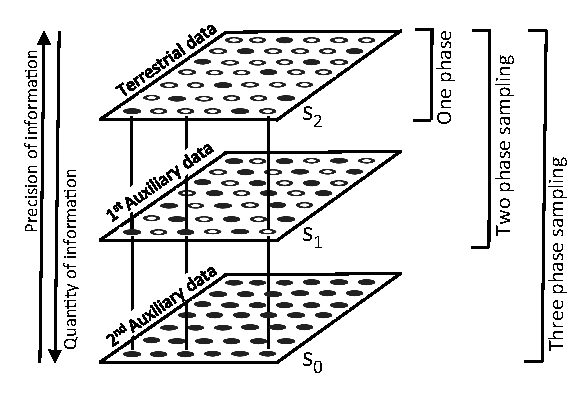
\includegraphics{Grafiken/Jstat_article/phases_graphic(new).eps}}%
		\caption{} \label{fig:concmphase_and_sae_a}
		\end{subfigure}
	\begin{subfigure}[t]{0.5\textwidth}
		\centering
	 \resizebox{0.58\hsize}{!}{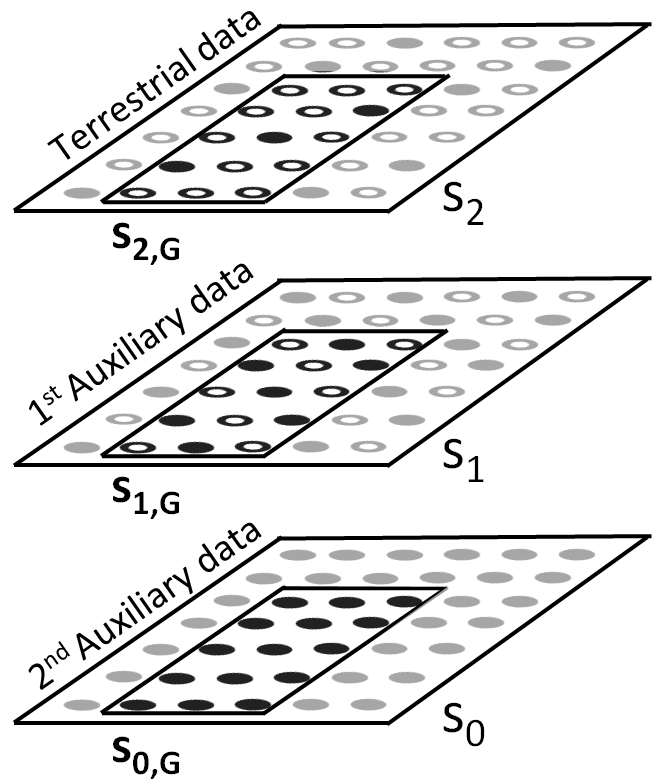
\includegraphics{Grafiken/Jstat_article/sae_graphic.PNG}}%
		\caption{} \label{fig:concmphase_and_sae_b}
	\end{subfigure}
\caption{(a) Concept of multi-phase sampling. The square represents the forest area for which an inventory is being conducted. The points denote the sample locations $x$. Filled points indicate available information. (b) Illustration of the small area estimation problem.}
\label{fig:concmphase_and_sae}
\end{figure}

\subsection{Small area estimation}

Small area estimation does not necessarily refer to small spatial areas but rather to areas that contain little or no terrestrial sample. To formulate this mathematically, we want to make an estimate for a subregion $G$ of the entire inventory area $F$ (Fig. \ref{fig:concmphase_and_sae_b}). As the sample size in the small area, $n_{2,G}$, is usually too small to provide sufficient estimation precision, multi-phase estimation can be efficient. However, $n_{2,G}$ may also be too small to justify fitting a separate regression model just for that area, because the estimates produce undesirably large confidence intervals. The idea is to borrow strength from the entire terrestrial sample $s_2$ of $F$ to fit the model, and then to apply this model to the small area. The potential bias of applying that model in $G$ is then corrected for by using the empirical model residuals derived from that small area. If there are no terrestrial plots in $G$ (i.e., $n_{2,G}=0$), one cannot correct for a potential model bias in $G$ and has to accept a potential bias in the estimator. These are called synthetic estimates. Despite their potential bias, it is usually still possible to calculate their design-based variance.


\subsection{Design-based vs. model-dependent approach}
\label{sec:db_vs_md}

The subject of model selection gets a lot of attention in the field of forest inventory. This is why it is important to understand that the mathematical interpretation of how a model is used to produce estimates is fundamentally different between the design-based and model-dependent approach. In the model-dependent (also known as model-based) framework, the sample locations $x$ are fixed and the observation $Y(x)$ taken at location $x$ is assumed to be a random variable as the forest is assumed to be the realization of a stochastic process. Although the model does not need to be fit from a probability sample, i.e., the sample locations could arbitrarily be chosen, the model should adequately describe the underlying stochastic process in order to efficiently ensure unbiased results. In practice this means that special attention must be made to ensure that the variable selection is appropriate to avoid overfitting, important variables are not omitted and all model assumptions are reasonably met through empirical verification. If a model is misspecified then estimation based on inference from that model may not be reliable. In the model-dependent framework one thus has to trust the model. In contrast, the design-based approach, on which all \pkg{forestinventory} estimators are based, rests upon the randomization of the sample locations $x$. While the sample locations $x$ are independently and uniformly distributed in the forest, the forest itself and thus the values of the local density surface at any location $x \in F$ are fixed and not the result of a stochastic process. A selected observation $Y(x)$ still remains a random variable, but solely due to the random sample mechanism. A consequence of this approach is that the estimation properties of design-based regression estimators (e.g., unbiasedness) typically hold regardless of the model that is chosen. The philosophy of the design-based approach is thus to use prediction models to improve the efficiency of the estimators without having to rely on their correct specification, which makes them very attractive to be used in official statistics. They are therefore also referred to as model-assisted. It should be noted that the randomization of sample locations upon which design-based inference depends, is in practice often replaced by systematic grids to minimize transportation costs in the terrestrial survey. However, there is reasonable evidence that softening this assumption is acceptable for point and variance estimation as long as the grid does not interact with periodic features in the forest structure \citep{mandallaz2008}. The variance will in most cases be slightly overestimated and lead to wider, more conservative confidence intervals \citep{mandallaz2013a}.

%\newpage

\subsection{Package structure}
\label{sec:packstruc}

In the \pkg{forestinventory} package, estimators for two-phase and three-phase sampling are applied with the \code{twophase()} and \code{threephase()} functions. From these two overall function calls, various estimators for specific inventory scenarios under the chosen sampling design can be applied (Fig. \ref{fig:struct_package}). Choosing an estimator follows a tree-like structure which can serve the user as a guideline throughout this article as well as in future applications. The basic decision to make is whether an estimate and its variance should be computed for an entire inventory area (global estimators) or only for subregions of the entire inventory area (small area estimators). In the second case, the package offers three small area estimators that will in detail be described in the following sections. The estimators are available under exhaustive and non-exhaustive use of the auxiliary data. Additionally, the package can also calculate one-phase estimates solely based on terrestrial samples. All estimators are also available for cluster sampling, in which case a sample unit consists of multiple, spatially agglomerated samples. The following sections describe the mathematical details and the application of the multi-phase estimators implemented in the \proglang{R} package \pkg{forestinventory}. While \cite{mandallaz2008, mandallaz2013techa, mandallaz2013techb,mandallaz2015tech} provides an extensive derivation of all estimators, we will provide the mathematical formulas that are actually implemented in the package. We will also restrict discussion to simple sampling, while the formulas for cluster sampling are available in the technical reports \citep{mandallaz2016, mandallaz2013techa, mandallaz2013techb}. A special case under cluster sampling is described in Section \ref{sec:speccas_and_scen}.

\begin{figure}[htb]
\centering
\resizebox{1\hsize}{!}{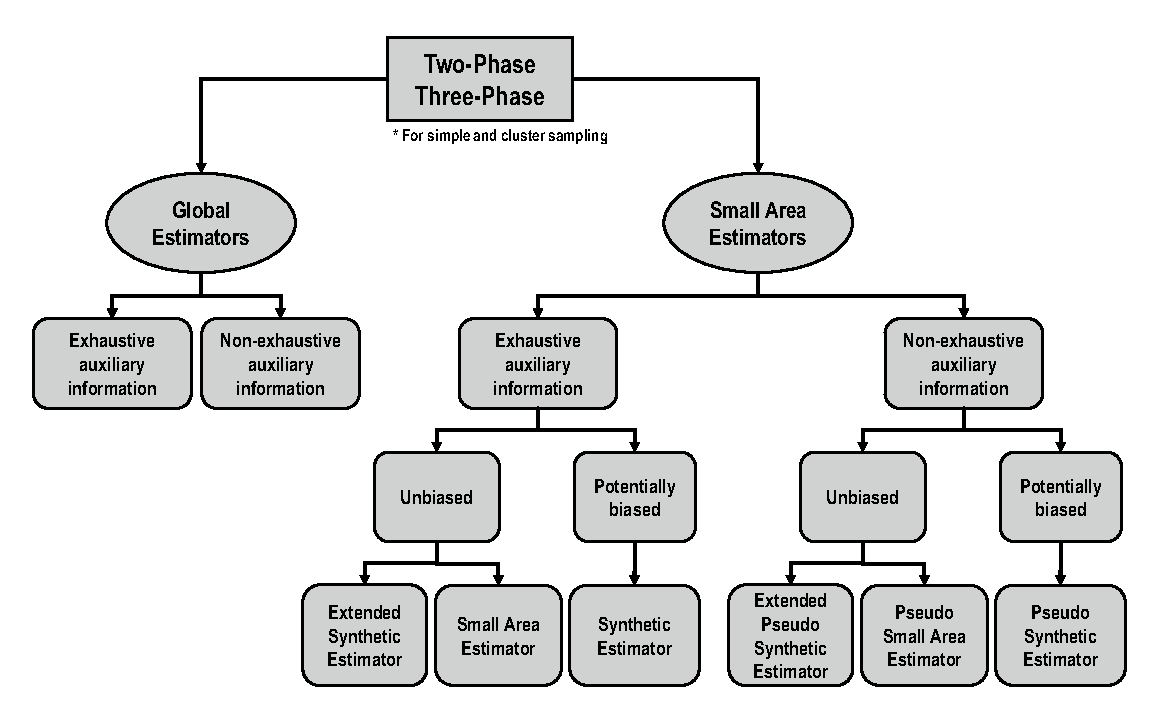
\includegraphics{Grafiken/Jstat_article/Package_structure_5.eps}}
\caption{Structure of the multi-phase estimators in the \proglang{R} package \pkg{forestinventory}. All estimators are also available for cluster sampling.}
\label{fig:struct_package}
\end{figure}

\newpage


%------------------------------------------------------------------------------------------------%
% ---------------------------------- Estimators and their Application -------------------------- %

\section{Two-phase estimators and their application}
\label{sec:twophase_and_appl}


% ---------------------------------------------------------------------------- %
\subsection{Global estimators}
\label{sec:twophase_globest}

\subsubsection{Mathematical background}

The vector of regression coefficients of the OLS regression model is found by using the following solution to the sample-based normal equation:

\begin{equation}\label{normequ_simple}
  \hat{\pmb{\beta}}_{s_2}=\Big(\frac{1}{n_2}\sum_{x\in{s_2}}\pmb{Z}(x)\pmb{Z}^{\top}(x) \Big)^{-1} \Big(\frac{1}{n_2}\sum_{x\in{s_2}}Y(x)\pmb{Z}(x)\Big)
\end{equation}

The individual predictions can then be calculated as $\hat{Y}(x)=\pmb{Z}^{\top}(x)\hat{\pmb{\beta}}_{s_2}$ and the empirical model residuals, which are only available at all sample locations $x \in s_2$, are calculated as $\hat{R}(x)=Y(x)-\hat{Y}(x)$. Unless stated otherwise, \pkg{forestinventory} only uses internal models to calculate estimates. This means that the model fit, i.e., $\hat{\pmb{\beta}}_{s_2}$, is derived from the current inventory data that are passed to the \code{twophase()} and \code{threephase()} functions.  While virtually all inventorists fit their models using the current inventory data, sometimes there is reason to use formulas derived from external models where the sample used to train the model is assumed to be taken from an independent source \citep{massey2015a}. However, this usually occurs when using a model other than the OLS regression model and is beyond the scope of the package at this time.\par

The package provides the calculation of point estimates under exhaustive (EX) and non-exhaustive (NEX) use of the auxiliary information, which means to respectively apply $\hat{\pmb{\beta}}_{s_2}$ to $\bar{\pmb{Z}}$, i.e., the exact spatial mean of $\pmb{Z}(x)$, or to $\hat{\bar{\pmb{Z}}}$, i.e., an estimate of the spatial mean of $\pmb{Z}(x)$:


\begin{subequations}\label{eq:pointest_2p_reg}
\begin{align}
  \hat{Y}_{reg2p,EX} & =\bar{\pmb{Z}}^{\top}\hat{\pmb{\beta}}_{s_2} \label{eq:pointest_2p_reg_ex}\\
  \hat{Y}_{reg2p,NEX} & =\hat{\bar{\pmb{Z}}}^{\top}\hat{\pmb{\beta}}_{s_2} \label{eq:pointest_2p_reg_nex}
\end{align}
\end{subequations}

Note that for internal linear models the mean of the empirical residuals $\frac{1}{n_2}\sum_{x\in{s_2}}\hat{R}(x)$ is zero by construction (zero mean residual property) which is why it does not appear in the point estimate. More explanation about how to obain the auxiliary means is given in the next subsection.

The \pkg{forestinventory} package implements two kinds of variances for each of these point estimates: the g-weight formulation that accounts for the fact that our model is in fact internal, and the external variance formulation that assumes a true external regression model and thus neglects the uncertainty in the regression coefficients \citep{mandallaz2016}.

The g-weight formulation is

\begin{subequations}\label{eq:gw_var_2p_reg}
\begin{align}
  \hat{\var}(\hat{Y}_{reg2p,EX}) & :=\bar{\pmb{Z}}^{\top}\hat{\pmb{\Sigma}}_{\hat{\pmb{\beta}}_{s_2}}\bar{\pmb{Z}} \label{eq:gw_var_2p_reg_ex}\\
  \hat{\var}(\hat{Y}_{reg2p,NEX}) & :=
  \hat{\bar{\pmb{Z}}}^{\top}\hat{\pmb{\Sigma}}_{\hat{\pmb{\beta}}_{s_2}}\hat{\bar{\pmb{Z}}}
  + \hat{\pmb{\beta}}_{s_2}^{\top}\hat{\pmb{\Sigma}}_{\hat{\bar{\pmb{Z}}}}\hat{\pmb{\beta}}_{s_2} \label{eq:gw_var_2p_reg_nex}
\end{align}
\end{subequations}

where the g-weight variance-covariance matrix of $\hat{\pmb{\beta}}_{s_2}$ is calculated as

\begin{equation}\label{eq:estvarmatrix}
  \hat{\pmb{\Sigma}}_{\hat{\pmb{\beta}}_{s_2}}:=\Big(\frac{1}{n_2}\sum_{x\in{s_2}}\pmb{Z}(x)\pmb{Z}^{\top}(x) \Big)^{-1}
  \Big(\frac{1}{n_2^2}\sum_{x\in{s_2}}\hat{R}^2(x)\pmb{Z}(x)\pmb{Z}^{\top}(x)\Big)
  \Big(\frac{1}{n_2}\sum_{x\in{s_2}}\pmb{Z}(x)\pmb{Z}^{\top}(x) \Big)^{-1}
\end{equation}

and the uncertainty caused by using the $s_1$ sample to estimate $\bar{\pmb{Z}}$ by $\hat{\bar{\pmb{Z}}}$ is accounted for by the variance-covariance matrix of the auxiliary vector $\hat{\bar{\pmb{Z}}}$
\begin{equation}\label{estvarcovaux}
\hat{\Sigma}_{\hat{\bar{\pmb{Z}}}}=
\frac{1}{n_{1}(n_{1}-1)}\sum_{x\in{s_{1}}}
(\pmb{Z}(x)-\hat{\bar{\pmb{Z}}})(\pmb{Z}(x)-\hat{\bar{\pmb{Z}}})^{\top}
\end{equation}

The external variance formulation for linear regression models is

\begin{subequations}\label{eq:varexternal_2p_reg}
\begin{align}
  \hat{\var}_{ext}(\hat{Y}_{reg2p,EX}) & = \frac{1}{n_2}\hat{\var}_{s_2}(\hat{R}(x)) \label{eq:varexternal_2p_reg_ex} \\
  \hat{\var}_{ext}(\hat{Y}_{reg2p,NEX}) & = \frac{1}{n_1}\hat{\var}_{s_1}(\hat{Y}(x)) + \frac{1}{n_2}\hat{\var}_{s_2}(\hat{R}(x)) \nonumber  \label{eq:varexternal_2p_reg_nex}
\end{align}
\end{subequations}
where $\hat{\var}_{s_2}$ and $\hat{\var}_{s_1}$ indicate taking the sample variance over $s_2$ and $s_1$ respectively.

Note that when applied to internal linear regression models, the external variance is asymptotically unbiased and usually slightly smaller than the g-weight variance, where the uncertainty of the regression coefficients is accounted for by the variance-covariance matrix (Eq. \ref{eq:estvarmatrix}).  The external variances are provided in the package \pkg{forestinventory} in case the user wants to compare linear models to another model type where no g-weight formulation is possible, as is the case with non-parametric models like kNN.

\subsubsection{Calculation of explanatory variables}

We will now draw our attention to the calculation of the explanatory variables from the auxiliary data for both the non-exhaustive and exhaustive cases. Fig. \ref{fig:exh_nexh_and_boundweights_b} depicts how the non-exhaustive case often looks like in practice: a regular terrestrial grid $s_2$ is given by a terrestrial inventory (the points surrounded by dotted circles) and densified to a larger sample $s_1$ (the points). For every point $x$, each explanatory variable in the vector $\pmb{Z}(x)=(z(x)_1, z(x)_2,...,z(x)_p)^{\top}$ is calculated using a defined spatial extent of auxiliary information around that point called the support (the dark green square tiles). We emphasize that the value of the explanatory variables for $\pmb{Z}(x)$ are associated with the sample point whereas the support is the spatial extent of the auxiliary information used to calculate those values. So far this is in perfect agreement with the presented theory of the non-exhaustive estimator, except for using regular grids rather than randomly placed sample points. The \pkg{forestinventory} package calculates the empirical mean of $\pmb{Z}(x)$ automatically from the input data frame using $\hat{\bar{\pmb{Z}}}=\frac{1}{n_{1}}\sum_{x\in{s_{1}}}\pmb{Z}(x)$.\par

The exhaustive case requires a closer look. In the infinite population approach, $\pmb{Z}(x)$ refers to the sample point $x$ and not the area around it. Deriving the exact spatial mean, $\bar{\pmb{Z}}=\frac{1}{\lambda(F)}\int_{F} \pmb{Z}(x)dx= (\frac{1}{\lambda(F)}\int_{F} z_1(x)dx, ..., \frac{1}{\lambda(F)}\int_{F} z_p(x)dx)^{\top}$, implies that we need to calculate the spatial mean of each component of $\pmb{Z}(x)$ using all possible points in $F$. This is much like the situation we had with calculating the mean of the local density surface for $Y(x)$ in that we need to find the mean of $\pmb{Z}(x)$ over an infinite number of sample points (i.e., $n_1=\infty$). Although it is practically infeasible to assess $\pmb{Z}(x)$ for every $x$, there are few cases where the exact mean can in fact be precisely calculated. The first case is when the explanatory variables are provided by polygon layers (e.g., map of development stages). In this case, one can calculate the exact mean as the area-weighted average of each categorical variable. The second case is when the exact mean can be calculated in one step, e.g., taking the mean of all height pixels of a raster canopy height model will perfectly equal the mean calculated by the use of an infinite number of supports \citep{mandallaz2013b}. However, for most types of explanatory variables we will try to get an approximation of $\bar{\pmb{Z}}$ that is only negligibly different. \par

One implementation to approximate the exact mean $\bar{\pmb{Z}}$ is shown in Fig. \ref{fig:exh_nexh_and_boundweights_a}, where the spatial arrangement of the supports (the dark green tiles) are tessellated to form a perfect partition over the inventory area in order for all of the wall-to-wall auxiliary information to be exploited. It has to be noted that this setup would allow for a perfect calculation of the exact mean $\bar{\pmb{Z}}$ in the finite population approach, i.e., deriving $\pmb{Z}(x)$ for the finite population of supports that are considered the sampling units. While in the infinite population approach this implementation probably does not produce the true exact mean $\bar{\pmb{Z}}$, $n_1$ is still expected to be reasonably large for the difference to be considered negligible as long as the size of the supports are not unreasonably large. However, the perfect tessellation implementation can also impose drawbacks. One is that a perfect tessellation by the supports strongly depends on the distance between the sample locations of $s_1$ and the support size. Since in practice the support size should ideally be chosen to achieve a best possible explanatory power of the regression model (thus minimizing the residual variation) a perfect tessellation might often not be feasible. In the infinite population frame, the supports are allowed to overlap if this seems necessary to acquire a sufficiently large sample $n_1$ to get a negligibly close approximation of $\bar{\pmb{Z}}$. With this respect, the infinite population approach provides more flexibility than the finite approach.

\begin{figure}[htb]
	\begin{subfigure}[t]{0.5\textwidth}
		\centering
    \resizebox{0.8\hsize}{!}{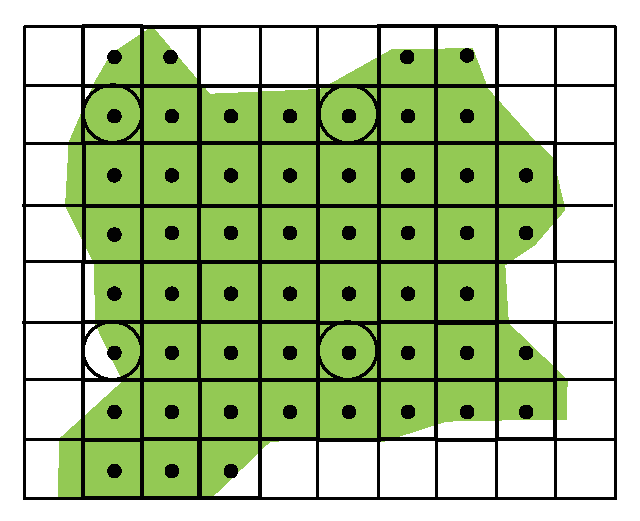
\includegraphics{Grafiken/Jstat_article/boundaryweight_graphic(left).eps}}%
		\caption{} \label{fig:exh_nexh_and_boundweights_a}
		\end{subfigure}
	\begin{subfigure}[t]{0.5\textwidth}
		\centering
   \resizebox{0.8\hsize}{!}{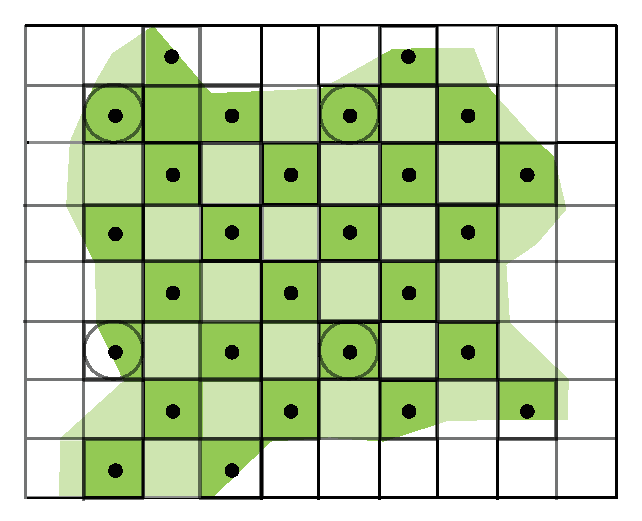
\includegraphics{Grafiken/Jstat_article/boundaryweight_graphic(right).eps}}%
		\caption{} \label{fig:exh_nexh_and_boundweights_b}
	\end{subfigure}
\caption{Concept of (a) exhaustive and (b) non-exhaustive calculation of explanatory variables including boundary adjustment at the support level. Auxiliary data are in both cases available over the entire inventory area marked by the large rectangle. A vector of explanatory variables $\pmb{Z}(x)$ is calculated within the supports (small squares)  at each sample location $x$ (points) that falls into the forest area (green underlying polygon).}
\label{fig:exh_nexh_bw}
\end{figure}

\subsubsection{Boundary adjustment}

An extension to the so-far published estimators by Mandallaz is the consideration of a boundary adjustment. In forest inventories, the sample is often restricted to those sample locations located within the forest area. In case a consistent forest definition can be applied to both the $s_2$ and $s_1$ sample (e.g., by a polygon forest mask layer), it might be desired to restrict the calculation of the explanatory variables to the forest area within the given support (see Fig. \ref{fig:exh_nexh_bw}). This method was suggested in \citet{mandallaz2013b} and led to an improvement in estimation precision. In order to ensure an unbiased calculation of either $\hat{\bar{\pmb{Z}}}$ or $\bar{\pmb{Z}}$, the respective means have then to be calculated as the weighted mean (Eq. \ref{eq:wmeanZ}) where the weight $w(x)$ is equal to the percentage of forested area within the support of sample location $x$.

\begin{equation}\label{eq:wmeanZ}
  \hat{\bar{\pmb{Z}}}=\frac{\sum_{x\in{s_1}}w(x)\pmb{Z}(x)}{\sum_{x\in{s_1}}w(x)}
\end{equation}

% --------------------------- %
\subsubsection{Application}

To demonstrate the use of the global two-phase estimators, we will use the \code{grisons} data set that comes with installing the package from the CRAN repository. The data set contains data from a simple (i.e., non-cluster) two-phase forest inventory conducted in 2007 that \citet{mandallaz2013b} used in a case study. The $s_1$ sample is comprised of 306 sample locations arranged on a systematic grid containing auxiliary information in the form of airborne laserscanning (ALS) canopy height metrics (\code{mean}, \code{stddev}, \code{max}, \code{q75}). For a systematic subsample of 67 ($s_2$ sample), terrestrial information of the timber volume per hectare (\code{tvol}) on the sample plot level is provided from a terrestrial survey. We can load \pkg{forestinventory} and examine the \code{grisons} data set in the \proglang{R} environment as follows:

\begin{small}
\begin{Schunk}
\begin{Sinput}
R> library("forestinventory")
R> data("grisons", package = "forestinventory")
R> head(grisons)
\end{Sinput}
\end{Schunk}
\end{small}

\begin{small}
\begin{Schunk}
\begin{Soutput}
   phase_id_2p boundary_weights  mean stddev   max   q75 smallarea   tvol
1            2             1.00  9.30  11.84 40.87 21.14         C 107.80
2            1             1.00 12.16  11.35 39.80 21.54         A     NA
3            2             1.00  5.25   5.74 23.82  9.53         D  63.77
4            1             1.00  7.53   9.33 34.10 13.02         A     NA
5            1             0.67  6.11   5.87 23.33 10.55         B     NA
6            1             1.00 12.15  10.16 33.76 20.97         C     NA
7            2             1.00  6.38   4.72 17.96 10.14         D 154.10
8            1             1.00  1.25   3.79 22.72  0.00         B     NA
9            1             1.00 21.56   7.49 32.66 27.81         A     NA
10           2             1.00 13.55   7.20 36.14 18.59         A 256.15
\end{Soutput}
\end{Schunk}
\end{small}

Estimates can be made using the \code{onephase()}, \code{twophase()} or \code{threephase()} functions. The data frame passed to these functions follows the tidy data structure \citep{wickham2014} where each row corresponds to an observation at a unique sample location and the columns specify the attributes associated to that respective sample location. Attributes that are missing, e.g., because they are associated with sample locations that were not selected in the subsample for the subsequent phase, should be designated as \code{NA} and the phase membership is encoded as numeric.

For global two-phase estimation, we have to specify

\begin{itemize}
  \itemsep0em
  \item the regression model (\code{formula}) as specified in the \code{lm}()-function \citep{R}.
  \item the passed \code{data.frame} containing the inventory information (\code{data}).
  \item the \code{list}-object \code{phase\_id} containing: the \code{phase.col} argument identifying the name of the column specifying membership to $s_1$ or $s_2$, and the \code{terrgrid.id} argument specifying which numeric value indicates $s_2$ membership in that column. Note that \pkg{forestinventory} implicitly assumes that all rows not indiscated as $s_2$ belong to the $s_1$ phase.
  \item the name of the column containing the weights $w(x)$ of the boundary adjustments (optional).
\end{itemize}

The non-exhaustive estimator with boundary weight adjustment can thus be applied as follows:

\begin{small}
\begin{Schunk}
\begin{Sinput}
R> reg2p_nex <- twophase(formula = tvol ~ mean + stddev + max + q75, data = grisons, 
+    phase_id = list(phase.col = "phase_id_2p", terrgrid.id = 2),
+    boundary_weights = "boundary_weights")
\end{Sinput}
\end{Schunk}
\end{small}

The \code{twophase()} function creates an \code{S3} object of class \code{"twophase"} with subclass \code{"global"}. A readable summary of the estimation results can be obtained by passing this object to the \code{summary()} function, which automatically interprets what type of estimator was used and returns pertinent information such as the regression model formula, the point estimate (\code{estimate}), the g-weight and external variance (\code{g\_variance} and \code{ext\_variance}) as well as the sample sizes and the model R$^2$:

\begin{small}
\begin{Schunk}
\begin{Sinput}
R> summary(reg2p_nex)
\end{Sinput}
\begin{Soutput}
Two-Phase global estimation
 
Call: 
twophase(formula = tvol ~ mean + stddev + max + q75, data = grisons, 
    phase_id = list(phase.col = "phase_id_2p", terrgrid.id = 2), 
    boundary_weights = "boundary_weights")

Method used:
Non-exhaustive global estimator
 
Regression Model:
tvol ~ mean + stddev + max + q75

Estimation results:
 estimate ext_variance g_variance  n1 n2 r.squared
 383.5354      279.954   271.5057 306 67 0.6428771

'boundary_weight'- option was used to calculate weighted means of auxiliary variables
\end{Soutput}
\end{Schunk}
\end{small}

% \begin{Schunk}
% \begin{Sinput}
% Two-Phase global estimation
%  
% Call: 
% twophase(formula = tvol ~ mean + stddev + max + q75, data = grisons, 
%     phase_id = list(phase.col = "phase_id_2p", terrgrid.id = 2), 
%     boundary_weights = "boundary_weights")
% 
% Method used:
% Non-exhaustive global estimator
%  
% Regression Model:
% tvol ~ mean + stddev + max + q75
% 
% Estimation results:
%  estimate ext_variance g_variance  n1 n2 r.squared
%  383.5354      279.954   271.5057 306 67 0.6428771
% 
% 'boundary_weight'- option was used to calculate weighted means of auxiliary variables
% \end{Sinput}
% \end{Schunk}

For practical use, one should normally always prefer the g-weight variance over the external variance, since for internal models, the regression coefficients actually depend on the terrestrial sample realized by the sampling design. In contrast to the external variance, the g-weight variance accounts for this sampling variability. This results in more reliable point and variance estimates and also benefits from better statistical calibration properties (g-weights). The external and g-weight variances are asymptotically equivalent but the external variance is really only included here in case the user wants to compare to another estimator where no g-weight variance exists.

The exhaustive estimator can be applied by additionally passing a vector containing the exact means of the explanatory variables, i.e., $\bar{\pmb{Z}}$, to the optional argument \code{exhaustive}. This vector must be calculated beforehand in such a way that any desired boundary adjustment has already been applied. Note that the vector input to \code{exhaustive} must be in the same order that the \code{lm()}-function processes a \code{formula} object including the intercept term whose exact mean will always be 1. Particular caution must be taken if categorical variables are present because the \code{lm()}-function, which is internally used to set up the design-matrix, automatically creates dummy variables with one of the categories used as a reference. Using our \code{grisons} example, the correct order can always be extracted by the following \proglang{R}-code:


\begin{small}
\begin{Schunk}
\begin{Sinput}
R> colnames(lm(formula = tvol ~ mean + stddev + max + q75, data = grisons, 
+    x = TRUE)$x)
\end{Sinput}
\end{Schunk}
\end{small}

The exhaustive estimator can be applied after defining the vector of exact means $\bar{\pmb{Z}}$ taken from \citet{mandallaz2013b}, denoted as \code{true.means.Z}:

\begin{small}
\begin{Schunk}
\begin{Sinput}
R> true.means.Z <- c(1, 11.39, 8.84, 32.68, 18.03)
R> reg2p_ex <- twophase(formula = tvol ~ mean + stddev + max + q75,
+    data = grisons,
+    phase_id = list(phase.col = "phase_id_2p", terrgrid.id = 2),
+    exhaustive = true.means.Z)
\end{Sinput}
\end{Schunk}
\end{small}

An alternative way to look at the estimation results without using the \code{summary()} is to query \code{reg2p\_ex} directly:
\begin{small}
\begin{Schunk}
\begin{Sinput}
R> reg2p_ex$estimation
\end{Sinput}
\begin{Soutput}
  estimate ext_variance g_variance  n1 n2 r.squared
1 376.7426     202.5602   187.2787 Inf 67 0.6428771
\end{Soutput}
\end{Schunk}
\end{small}
Note that both variances of the exhaustive estimation are smaller than those of the non-exhaustive estimation. This is essentially because we eliminated one component of uncertainty by substituting the estimated means of the explanatory variables $\hat{\bar{\pmb{Z}}}$ by their exact means $\bar{\pmb{Z}}$.


%--------------------------------------------------------------------------------------------------%
% ################################################################################################ %
%--------------------------------------------------------------------------------------------------%

\subsection{Small area estimators}
\label{sec:twophase_sae}

\subsubsection{Mathematical background}

The \pkg{forestinventory} package provides three types of small area estimators each of which has an exhaustive and non-exhaustive form. We will use a different nomenclature for the non-exhaustive case in small area estimation since much of the existing literature shows preference for the label pseudo to indicate that the mean of the explanatory variables within the small area was based on a finite sample. The main idea for all these small area estimators is to calculate the regression coefficient vector $\hat{\pmb{\beta}}_{s_2}$ and its variance-covariance matrix $\hat{\pmb{\Sigma}}_{\hat{\pmb{\beta}}_{s_2}}$ on the entire $s_2$ sample according to Eq. \ref{normequ_simple} and \ref{eq:estvarmatrix}, and subsequently use that to make predictions for sample locations restricted to small area $G$.\par

%----------------------------------------------- %
% \textbf{Small and Pseudo Small Area Estimator}\par

We first introduce the small area estimator (SMALL), which uses exhaustively computed explanatory variables, and its non-exhaustive version, the pseudo small area estimator (PSMALL). 

\begin{subequations}\label{eq:pest_2p_small_psmall}
\begin{align}
  \hat{Y}_{G,SMALL,2p} & =\bar{\pmb{Z}}_G^{\top}\hat{\pmb{\beta}}_{s_2} + \frac{1}{n_{2,G}}\hat{R}(x)  \label{eq:pointest_2p_small} \\
  \hat{Y}_{G,PSMALL,2p} & =\hat{\bar{\pmb{Z}}}_G^{\top}\hat{\pmb{\beta}}_{s_2} + \frac{1}{n_{2,G}}\hat{R}(x) \label{eq:pepsmall}
\end{align}
\end{subequations}

In the equations for the point estimates (Eq. \ref{eq:pointest_2p_small} and \ref{eq:pepsmall}), we see that the globally derived regression coefficients are applied to the exhaustively or non-exhaustively calculated means of the explanatory variables ($\bar{\pmb{Z}}_G$, $\hat{\bar{\pmb{Z}}}_G$) which are now only based on the first-phase sample $s_{1,G}$ located within small area $G$. A potential bias of the regression model predictions in the small area $G$, due to fitting the regression model with data also outside of $G$, is then corrected by adding the mean of the empirical model residuals in $G$. This is called the bias or residual correction term.

The package provides the g-weight variance for SMALL and PSMALL respectively (Eq. \ref{eq:var_2p_reg_small}, \ref{eq:var_2p_reg_psmall}) as well as the  external variance (Eq. \ref{eq:varext_2p_reg_small}, \ref{eq:varext_2p_reg_psmall}). Again note that all components are restricted to those available at the sample locations in the small area ($s_{1,G}$ and $s_{2,G}$), with exception of the regression coefficient components $\hat{\pmb{\beta}}_{s_2}$ and $\hat{\pmb{\Sigma}}_{\hat{\pmb{\beta}}_{s_2}}$.


\begin{subequations}\label{eq:var_2p_small_psmall}
\begin{align}
  \hat{\var}(\hat{Y}_{G,SMALL,2p}) & := \bar{\pmb{Z}}_G^{\top}\hat{\pmb{\Sigma}}_{\hat{\pmb{\beta}}_{s_2}}\bar{\pmb{Z}}_G
    + \frac{1}{n_{2,G}}\hat{\var}_{s_{2,G}}(\hat{R}(x))  \label{eq:var_2p_reg_small} \\
  \hat{\var}(\hat{Y}_{G,PSMALL,2p}) & := \hat{\bar{\pmb{Z}}}_G^{\top}\hat{\pmb{\Sigma}}_{\hat{\pmb{\beta}}_{s_2}}\hat{\bar{\pmb{Z}}}_G
  + \hat{\pmb{\beta}}_{s_2}^{\top}\hat{\Sigma}_{\hat{\bar{\pmb{Z}}}_G}\hat{\pmb{\beta}}_{s_2}
  + \frac{1}{n_{2,G}}\hat{\var}_{s_{2,G}}(\hat{R}(x))  \label{eq:var_2p_reg_psmall}
\end{align}
\end{subequations}

\begin{subequations}\label{eq:varext_2p_small_psmall}
\begin{align}
  \hat{\var}_{ext}(\hat{Y}_{G,SMALL,2p}) & := \frac{1}{n_{2,G}}\hat{\var}_{s_{2,G}}(\hat{R}(x))  \label{eq:varext_2p_reg_small} \\
  \hat{\var}_{ext}(\hat{Y}_{G,PSMALL,2p}) & := \frac{1}{n_{1,G}}\hat{\var}_{s_{2,G}}(Y(x)) + \Big(1-\frac{n_{2,G}}{n_{1,G}}\Big)\frac{1}{n_{2,G}}\hat{\var}_{s_{2,G}}(\hat{R}(x)) \label{eq:varext_2p_reg_psmall}
\end{align}
\end{subequations}
where $\hat{\var}_{s_{2,G}}$ indicates taking the sample variance over $s_{2,G}$. If boundary adjustment is applied, the simple mean of the explanatory variable vector over the small area $\hat{\bar{\pmb{Z}}}_G=\frac{1}{n_{1,G}}\sum_{x \in s_{1,G}}\pmb{Z}(x)$ is replaced by its weighted version $\hat{\bar{\pmb{Z}}}_G=\frac{\sum_{x\in{s_{1,G}}}w(x)\pmb{Z}(x)}{\sum_{x\in{s_{1,G}}}w(x)}$, and likewise for exhaustively used auxiliary information.



%------------------------------------------------------------- %
% \textbf{Synthetic and Pseudo Synthetic Estimator}\par

The synthetic estimator (SYNTH) and pseudo synthetic estimator (PSYNTH) are commonly applied when no terrestrial sample is available within the small area $G$ (i.e., $n_{2,G}=0$). In this case, the point estimates (Eq. \ref{eq:pointest_2p_reg_synth} and \ref{eq:pointest_2p_reg_psynth}) are based only on the predictions generated by applying the globally derived regression model to the auxiliary vectors $\bar{\pmb{Z}}_G$ and $\hat{\bar{\pmb{Z}}}_G$ respectively. However, the bias correction using the observed residuals $\hat{R}(x)$ is not applied as was the case in the small and pseudo small area estimator (Eq. \ref{eq:pointest_2p_small} and \ref{eq:pepsmall}). Thus, the (pseudo) synthetic estimator has a potentially unobservable design-based bias. Also note that the residual variation can no longer be considered in the g-weight variance (Eq. \ref{eq:var_2p_reg_synth} and \ref{eq:var_2p_reg_psynth}). Therefore, the synthetic estimators will usually have a smaller variance than estimators incorporating the regression model uncertainties, but at the cost of a potential bias. Due to the absence of available residuals in $G$, there is also no external variance form for the synthetic and pseudo synthetic estimator.

% Left out for simplicity reasons in article, maybe include in Diss:
% However, this assumption is unlikely to be fullfilled in practice resulting in a potentially unobservable design-based bias equal to $-\frac{1}{\lambda(G)}\int_G R(x)$. 

\begin{subequations}\label{eq:pest_2p_synth_psynth}
\begin{align}
  \hat{Y}_{G,SYNTH,2p} & =\bar{\pmb{Z}}_G^{\top}\hat{\pmb{\beta}}_{s_2} \label{eq:pointest_2p_reg_synth} \\
  \hat{Y}_{G,PSYNTH,2p} & =\hat{\bar{\pmb{Z}}}_G^{\top}\hat{\pmb{\beta}}_{s_2} \label{eq:pointest_2p_reg_psynth} \\
  \hat{\var}(\hat{Y}_{G,SYNTH,2p}) & = \bar{\pmb{Z}}_G^{\top}\hat{\pmb{\Sigma}}_{\hat{\pmb{\beta}}_{s_2}}\bar{\pmb{Z}}_G \label{eq:var_2p_reg_synth} \\
  \hat{\var}(\hat{Y}_{G,PSYNTH,2p}) & = \hat{\bar{\pmb{Z}}}_G^{\top}\hat{\pmb{\Sigma}}_{\hat{\pmb{\beta}}_{s_2}}\hat{\bar{\pmb{Z}}}_G
  + \hat{\pmb{\beta}}_{s_2}^{\top}\hat{\pmb{\Sigma}}_{\hat{\bar{\pmb{Z}}}_G}\hat{\pmb{\beta}}_{s_2}  \label{eq:var_2p_reg_psynth}
\end{align}
\end{subequations}

where the variance-covariance matrix of the auxiliary vector $\hat{\bar{\pmb{Z}}}_G$ is estimated by
\begin{equation}\label{estvarcovaux_G}
\hat{\Sigma}_{\hat{\bar{\pmb{Z}}}_{G}}=
\frac{1}{n_{1,G}(n_{1,G}-1)}\sum_{x\in{s_{1,G}}}
(\pmb{Z}(x)-\hat{\bar{\pmb{Z}}}_{G})(\pmb{Z}(x)-\hat{\bar{\pmb{Z}}}_{G})^{\top}
\end{equation}

%------------------------------------------------------------- %
% \textbf{Extended Synthetic and Extended Pseudo Synthetic Estimator}\par

The synthetic estimators, SYNTH and PSYNTH, have attractively compact formulas but come with the downside of potential bias in their point estimates which can make the variances seem deceptively optimistic. The SMALL and PSMALL estimators overcome this issue by using a bias correction term, i.e., $\frac{1}{n_{2,G}}\sum_{x \in s_{2,G}}\hat{R}(x)$. The motivation behind the extended synthetic and extended pseudo synthetic estimator (EXTSYNTH and EXTPSYNTH) is to use the same mathematically elegant formulas of the (pseudo) synthetic estimators while ensuring that the mean of the empirical prediction model residuals in the entire area $F$ and the small area $G$ are by construction both zero at the same time. This is accomplished by extending the vector of auxiliary information $\pmb{Z}(x)$ by a binary categorical indicator variable $I_G(x)$ which takes the value 1 if the sample location $x$ lies inside the target small area $G$ and is otherwise set to 0. Recalling that linear models fitted using OLS have zero mean residual property by construction also if categorical variables are used, this leads to unbiased point estimates. The new extended auxiliary vector thus becomes $\pmb{\mathbb{Z}}^{\top}(x)=(\pmb{Z}^{\top}(x),I^{\top}_G(x))$ and can be used to replace its non-extended counterpart $\pmb{Z}^{\top}(x)$ whereever it is used in Eq. \ref{eq:pest_2p_synth_psynth} and \ref{estvarcovaux_G}. Note that the package functions internally extend the data set by the indicator variable if the EXTSYNTH or EXTPSYNTH estimator is called.

Not every equation needs to be re-written here, but to give an example of the notational change, the regression coefficient under extended model approach becomes

\begin{equation}\label{ext_normequ_simple}
  \hat{\pmb{\theta}}_{s_2}=\Big(\frac{1}{n_2}\sum_{x\in{s_2}}\pmb{\mathbb{Z}}(x)\pmb{\mathbb{Z}}^{\top}(x) \Big)^{-1} \Big(\frac{1}{n_2}\sum_{x\in{s_2}}Y(x)\pmb{\mathbb{Z}}(x)\Big)
\end{equation}

The point estimates and their g-weight variances can then be re-written as

\begin{subequations}\label{eq:pest_2p_extsynth_extpsynth}
\begin{align}
\hat{Y}_{G,EXTSYNTH,2p} & = \bar{\pmb{\mathbb{Z}}}^{\top}_{G}\hat{\pmb{\theta}}_{s_2} \label{eq:pointest_2p_extsynth} \\
\hat{Y}_{G,EXTPSYNTH,2p} & =\hat{\bar{\pmb{\mathbb{Z}}}}_{G}^{\top}\hat{\pmb{\theta}}_{s_2} \label{eq:pointest_2p_extsynth} \\
\hat{\var}(\hat{Y}_{G,EXTSYNTH,2p}) & = \bar{\pmb{\mathbb{Z}}}^{\top}_{G}\hat{\pmb{\Sigma}}_{\hat{\pmb{\theta}}_{s_2}}\bar{\pmb{\mathbb{Z}}}_{G} \label{eq:var_2p_extsynth} \\
\hat{\var}(\hat{Y}_{G,EXTPSYNTH,2p})& =
\hat{\bar{\pmb{\mathbb{Z}}}}_{G}^{\top}\hat{\pmb{\Sigma}}_{\hat{\pmb{\theta}}_{s_2}}
\hat{\bar{\pmb{\mathbb{Z}}}}_{G}
+ \hat{\pmb{\theta}}^{\top}_{s_2}\hat{\pmb{\Sigma}}_{\hat{\bar{\pmb{\mathbb{Z}}}}_{G}}\hat{\pmb{\theta}}_{s_2} \label{eq:var_2p_extpsynth}
\end{align}
\end{subequations}

While the formulas look similar to the synthetic estimators, note that a decomposition of $\hat{\pmb{\theta}}_{s_2}$ reveals that the residual correction term is now included in the regression coefficient $\hat{\pmb{\theta}}_{s_2}$ \citep{mandallaz2016} and thus the estimates are asymptotically design-unbiased.

The package also provides the external variance for both the extended synthetic and extended pseudo synthetic estimator. Note that neither the extended model approach nor external variance estimates are possible in the absence of terrestrial samples and thus model residuals in $G$, which is precisely when one must rely on the (pseudo) synthetic estimates. The external variance forms of EXTSYNTH and EXTPSYNTH are

\begin{subequations}\label{eq:ext_varexternal_2p_extsynth}
\begin{align}
  \hat{\var}_{ext}(\hat{Y}_{G,EXTSYNTH,2p}) & = \frac{1}{n_{2,G}}\hat{\var}_{s_{2,G}}(\hat{\mathbb{R}}(x)) \label{eq:ext_varexternal_2p_extsynth} \\
  \hat{\var}_{ext}(\hat{Y}_{G,EXTPSYNTH,2p}) & = \frac{1}{n_{1,G}}\hat{\var}_{s_{2,G}}(Y(x)) + \Big(1-\frac{n_{2,G}}{n_{1,G}}\Big)\frac{1}{n_{2,G}}\hat{\var}_{s_{2_G}}(\hat{\mathbb{R}}(x)) \label{eq:ext_varexternal_2p_extpsynth}
\end{align}
\end{subequations}
where $\hat{\mathbb{R}}(x)$ are the empirical residuals under the extended auxiliary vector.

To summarize, the synthetic estimators SYNTH and PSYNTH can be applied whether terrestrial inventory sample is found in the small area or not, but has a deceptively small g-weight variance due to its potential bias.  When terrestrial sample is observed in the small area, we can produce (asymptotically) design-unbiased estimates and variances using either SMALL or PSMALL which remove this bias explicitly with a mean residual term, or more elegantly with EXTSYNTH or EXTPSYNTH which simply use the same synthetic formulas while including an indicator variable for the small area in the model formula to remove the bias by construction in OLS.


%------------------------------------------------------------- %
\subsubsection{Application}

Small area estimates in the \pkg{forestinventory} package can be applied by specifying the optional argument \code{small\_area}. The input data set has to include an additional column of class \code{factor} that describes the small area membership of the sample location represented by that row. The argument \code{small\_area} requires a \code{list}-object that comprises

\begin{itemize}
  \itemsep0em
  \item the name of the column specifiying the small area of each observation (\code{sa.col}).
  \item a vector specifying the small area(s) for which estimations are desired (\code{areas}).
  \item the argument \code{unbiased} that controls which of the three available estimators is applied.
\end{itemize}

In order to apply the pseudo small area estimator (PSMALL) with boundary adjustment, we set \code{unbiased=TRUE} as well as the optional argument \code{psmall=TRUE}:
\begin{small}
\begin{Schunk}
\begin{Sinput}
R> psmall_2p <- twophase(formula = tvol ~ mean + stddev + max + q75, 
+    data = grisons, phase_id = list(phase.col = "phase_id_2p", terrgrid.id = 2),
+    small_area = list(sa.col = "smallarea", areas = c("A", "B"),
+    unbiased = TRUE), psmall = TRUE, boundary_weights = "boundary_weights")
\end{Sinput}
\end{Schunk}
\end{small}

\begin{small}
\begin{Schunk}
\begin{Sinput}
R> summary(psmall_2p)
\end{Sinput}
\begin{Soutput}
Two-phase small area estimation
 
Call: 
twophase(formula = tvol ~ mean + stddev + max + q75, data = grisons, 
    phase_id = list(phase.col = "phase_id_2p", terrgrid.id = 2), 
    small_area = list(sa.col = "smallarea", areas = c("A", "B"), 
        unbiased = TRUE), boundary_weights = "boundary_weights", 
    psmall = TRUE)

Method used:
Pseudo small area estimator
 
Regression Model:
tvol ~ mean + stddev + max + q75

Estimation results:
 area estimate ext_variance g_variance  n1 n2 n1G n2G r.squared
    A 393.9713     1009.034   1308.117 306 67  94  19 0.6428771
    B 419.6416     1214.035   1259.472 306 67  81  17 0.6428771

'boundary_weight'- option was used to calculate weighted means of auxiliary variables
\end{Soutput}
\end{Schunk}
\end{small}

The small area functions all return an \code{S3} object of class \code{"twophase"} with subclass \code{"smallarea"}. In addition to global estimation, the \code{estimation} object now comprises the estimates and variances for all small areas (column \code{area}). We can view the sample sizes by looking into the object itself
\begin{small}
\begin{Schunk}
\begin{Sinput}
R> psmall_2p$samplesizes
\end{Sinput}
\begin{Soutput}
$A
      n1G n2G  n1 n2
plots  94  19 306 67

$B
      n1G n2G  n1 n2
plots  81  17 306 67
\end{Soutput}
\end{Schunk}
\end{small}

The extended pseudo synthetic estimator (EXTPSYNTH) can be applied by setting \code{unbiased=TRUE} and leaving the optional argument \code{psmall} to its default value of \code{FALSE}:


\begin{small}
\begin{Schunk}
\begin{Sinput}
R> extpsynth_2p <- twophase(formula = tvol ~ mean + stddev + max + q75, 
+    data = grisons, phase_id = list(phase.col = "phase_id_2p", terrgrid.id = 2),
+    small_area = list(sa.col = "smallarea", areas = c("A", "B"),
+    unbiased = TRUE), boundary_weights = "boundary_weights")
R> extpsynth_2p$estimation
\end{Sinput}
\begin{Soutput}
  area estimate ext_variance g_variance  n1 n2 n1G n2G r.squared
1    A 391.9356     995.5602   1017.633 306 67  94  19 0.6526503
2    B 419.7231    1214.6053   1019.191 306 67  81  17 0.6428854
\end{Soutput}
\end{Schunk}
\end{small}

The \pkg{forestinventory} package automatically includes the indicator variable for the small area behind the scenes so there is no need for the user to implement it. Notice that the $R^2$ values (\code{r.squared}) under the EXTPSYNTH estimator vary between the small areas, while they are identical under the PSMALL estimator. This is because under the EXTPSYNTH estimator, the regression model is recalculated for each small area estimation after adding the indicator variable for the respective small area in the globally derived design matrix. In case of the PSMALL estimator, the regression model stays the same for each small area estimation. Although the results of both estimators should always be close to each other, we recommend applying both estimators and compare the results afterwards in order to reveal unsuspected patterns in the data, particularly in the case of cluster sampling (see Section \ref{sec:speccas_and_scen}).\par

Setting the argument \code{unbiased=FALSE} applies the pseudo synthetic estimator to the selected small areas. Note that in the \code{grisons} data set, all small areas possess much more than the suggested minimum number of terrestrial observations (a rule of thumb is that $n_{2,G} \geq 6$) required to produce reliable design-unbiased estimates. Hence, choosing to use PSYNTH is probably not desireable and is just applied here for demonstration purposes. In this case the residual correction will not be applied.


\begin{small}
\begin{Schunk}
\begin{Sinput}
R> psynth_2p <- twophase(formula = tvol ~ mean + stddev + max + q75, 
+    data = grisons, phase_id = list(phase.col = "phase_id_2p", terrgrid.id = 2),
+    small_area = list(sa.col = "smallarea", areas = c("A", "B"),
+    unbiased = FALSE), boundary_weights = "boundary_weights")
\end{Sinput}
\end{Schunk}
\end{small}

\begin{small}
\begin{Schunk}
\begin{Sinput}
R> psynth_2p$estimation
\end{Sinput}
\begin{Soutput}
  area estimate ext_variance g_variance  n1 n2 n1G n2G r.squared
1    A 421.8863           NA   546.8651 306 67  94  19 0.6428771
2    B 418.7399           NA   566.3361 306 67  81  17 0.6428771
\end{Soutput}
\end{Schunk}
\end{small}

We see here that the PSYNTH variances are almost only half the variances of the PSMALL and EXTPSYNTH estimator. However, PSMALL and EXTPSYNTH are design unbiased and their variances reflect the fact that they account for potential bias of the regression model predictions. The g-weight variance of PSYNTH completely neglects a potential bias and as a result risks severely overstating the estimation precision.\par

The exhaustive versions of the small area estimators (Eq. \ref{eq:pointest_2p_small}, \ref{eq:var_2p_reg_small}, \ref{eq:varext_2p_reg_small}, \ref{eq:pointest_2p_reg_synth}, \ref{eq:var_2p_reg_synth}) are specified via the optional argument \code{exhaustive}. Its application requires that we know the exact means of all explanatory variables within the small area(s) of interest. In contrast to the global estimators, the exact means have now to be delivered in the form of a \code{data.frame}, where each row corresponds to a small area, and each column specifies the exact mean of the respective explanatory variable. Note that likewise the case of global estimation, the order of the explanatory variables in the data frame has to match the order in which they appear in the design matrix defined by the \code{lm()}-function in \proglang{R}. In order to tell \proglang{R} which row describes which small area, the row names have to match the respective names of the small areas specified in the \code{areas} argument.

For the \code{grisons} data set, the exact means of the explanatory variables for the small areas used in \citet{mandallaz2013b} are thus defined by
\begin{small}
\begin{Schunk}
\begin{Sinput}
R> colnames(lm(formula = tvol ~ mean + stddev + max + q75, data = grisons, 
+    x = TRUE)$x)
\end{Sinput}
\end{Schunk}
\end{small}
\begin{small}
\begin{Schunk}
\begin{Sinput}
R> true.means.Z.G <- data.frame(Intercept = rep(1, 4),
+    mean = c(12.85, 12.21, 9.33, 10.45),
+    stddev = c(9.31, 9.47, 7.90, 8.36),
+    max = c(34.92, 35.36, 28.81, 30.22),
+    q75 = c(19.77, 19.16, 15.40, 16.91))
R> rownames(true.means.Z.G) <- c("A", "B", "C", "D")
\end{Sinput}
\end{Schunk}
\end{small}
\begin{small}
\begin{Schunk}
\begin{Sinput}
R> true.means.Z.G
\end{Sinput}
\begin{Soutput}
  Intercept  mean stddev   max   q75
A         1 12.85   9.31 34.92 19.77
B         1 12.21   9.47 35.36 19.16
C         1  9.33   7.90 28.81 15.40
D         1 10.45   8.36 30.22 16.91
\end{Soutput}
\end{Schunk}
\end{small}

The extended synthetic estimator (EXTSYNTH) can then be applied by
\begin{small}
\begin{Schunk}
\begin{Sinput}
R> extsynth_2p <- twophase(formula = tvol ~ mean + stddev + max + q75, 
+    data = grisons, phase_id = list(phase.col = "phase_id_2p", terrgrid.id = 2),
+    small_area = list(sa.col ="smallarea", areas = c("A", "B"),
+    unbiased = TRUE), exhaustive = true.means.Z.G)
\end{Sinput}
\end{Schunk}
\end{small}

\begin{small}
\begin{Schunk}
\begin{Sinput}
R> extsynth_2p$estimation
\end{Sinput}
\begin{Soutput}
  area estimate ext_variance g_variance  n1 n2 n1G n2G r.squared
1    A 372.6930     744.3658   696.5739 Inf 67 Inf  19 0.6526503
2    B 387.5116     693.8576   708.1105 Inf 67 Inf  17 0.6428854
\end{Soutput}
\end{Schunk}
\end{small}

Just as in the global case, we see that the variance has again been significantly decreased by substituting the exact auxiliary means and both first phase sample sizes are now infinity. Note that the function extracts the required exact means for small area \code{"A"} and \code{"B"} from the complete set of exact means defined in \code{true.means.Z.G}.

\newpage

\section{Three-phase estimators and their application}
\label{sec:threephase_and_appl}

% ---------------------------------------------------------------------------- %
% ---------------------------------------------------------------------------- %
\subsection{Global estimators}
\label{sec:glob_est_3p}


% ------------------------------------- %
\subsubsection{Mathematical background}


Solving the sample-based normal equations, the vector of regression coefficients $\hat{\pmb{\alpha}}_{s_2}$ for the reduced model, i.e., using the reduced set of explanatory variables $\pmb{Z}^{(0)}(x)$ available at $x \in s_0$, and likewise the vector of regression coefficients $\hat{\pmb{\beta}}_{s_2}$ for the full model, i.e., using the full set of explanatory variables $\pmb{Z}^{\top}(x)=(\pmb{Z}^{(0)\top}(x),\pmb{Z}^{(1)\top}(x))$ available only at a subset $x \in s_1 \subset s_0$, are derived as

\begin{subequations}\label{eq:normequ_3p}
\begin{align}
\hat{\pmb{\alpha}}_{s_2}&=\Big(\frac{1}{n_2}\sum_{x\in{s}_2}\pmb{Z}^{(0)}(x)\pmb{Z}^{(0)\top}(x)
\Big)^{-1}\frac{1}{n_2}\sum_{x\in{s}_2}Y(x)\pmb{Z}^{(0)}(x)  \label{eq:normequ_redmod} \\
\hat{\pmb{\beta}}_{s_2}&=\Big(\frac{1}{n_2}\sum_{x\in{s}_2}\pmb{Z}(x)\pmb{Z}^{\top}(x)
\Big)^{-1}\frac{1}{n_2}\sum_{x\in{s}_2}Y(x)\pmb{Z}(x) \label{eq:normequ_fullmod}
\end{align}
\end{subequations}

The package allows for the calculation of point estimates under exhaustive and non-exhaustive use of the auxiliary information in the $s_0$ phase. Fitting the model using $s_2$ (i.e., internally) ensures the zero mean residual property over $s_2$.

\begin{subequations}\label{eq:reg3p}
\begin{align}
\hat{Y}_{reg3p,EX}&=\frac{1}{\lambda(F)}\int_{F} \pmb{Z}^{(0)\top}(x)\hat{\pmb{\alpha}}_{s_2} + \frac{1}{n_1}\sum_{x\in s_1} (\pmb{Z}^{\top}(x)\hat{\pmb{\beta}}_{s_2}-\pmb{Z}^{(0)\top}(x)\hat{\pmb{\alpha}}_{s_2}) + \frac{1}{n_2}\sum_{x\in s_2}(Y(x)-\pmb{Z}^{\top}(x)\hat{\pmb{\beta}}_{s_2})
\nonumber \\&= (\bar{\pmb{Z}}^{(0)}_0-\hat{\bar{\pmb{Z}}}^{(0)}_1)^{\top}\hat{\pmb{\alpha}}_{s_2} +
\hat{\bar{\pmb{Z}}}^{\top}_1\hat{\pmb{\beta}}_{s_2} \label{eq:reg3p_ex} \\
\hat{Y}_{reg3p,NEX}&=\frac{1}{n_0}\sum_{x\in s_0} \pmb{Z}^{(0)\top}(x)\hat{\pmb{\alpha}}_{s_2} + \frac{1}{n_1}\sum_{x\in s_1} (\pmb{Z}^{\top}(x)\hat{\pmb{\beta}}_{s_2}-\pmb{Z}^{(0)\top}(x)\hat{\pmb{\alpha}}_{s_2}) + \frac{1}{n_2}\sum_{x\in s_2}(Y(x)-\pmb{Z}^{\top}(x)\hat{\pmb{\beta}}_{s_2})
\nonumber \\&=(\hat{\bar{\pmb{Z}}}^{(0)}_0-\hat{\bar{\pmb{Z}}}^{(0)}_1)^{\top}\hat{\pmb{\alpha}}_{s_2}  +
\hat{\bar{\pmb{Z}}}^{\top}_1\hat{\pmb{\beta}}_{s_2} \label{eq:reg3p_nex}
\end{align}
\end{subequations}

Intuitively, the three phase estimator is simply the mean of the predictions using the reduced model, corrected by the mean difference between the reduced model predictions and the more accurate full model predictions, corrected by the mean difference between the ground truth and the full model predictions. For the compact version of the formula in the non-exhaustive case, the estimated means of $\pmb{Z}^{(0)}(x)$ over both the $s_0$ and $s_1$ phase, as well as the estimated mean of $\pmb{Z}(x)$ over the $s_1$ phase are calculated according to Eq. \ref{meanvalues3pnex}. If the exact mean over $s_0$ is known, the estimated mean $\hat{\bar{\pmb{Z}}}^{(0)}_0$ can simply be replaced by the exact mean $\bar{\pmb{Z}}^{(0)}_0$. Note that in case of applied boundary adjustment (Section \ref{sec:twophase_and_appl}), the simple mean is again replaced by the weighted mean analogous to Eq. \ref{eq:wmeanZ}.

\begin{equation}\label{meanvalues3pnex}
\hat{\bar{\pmb{Z}}}^{(0)}_0=\frac{1}{n_0}\sum_{x\in{s_0}} \pmb{Z}^{(0)}(x), \quad \hat{\bar{\pmb{Z}}}^{(0)}_1=\frac{1}{n_1}\sum_{x\in{s}_1}\pmb{Z}^{(0)}(x) ,
\quad \hat{\bar{\pmb{Z}}}_1=\frac{1}{n_1}\sum_{x\in{s}_1}\pmb{Z}(x)
\end{equation}

The package again provides the g-weight and external variances. The g-weight variance formulation is

\begin{subequations}\label{eq:dbvar_reg3p}
\begin{align}
\hat{\var}(\hat{Y}_{reg3p,EX})& =\frac{n_2}{n_1}\bar{\pmb{Z}}^{(0)\top}\hat{\pmb{\Sigma}}_{\hat{\pmb{\alpha}}_{s_2}}
\bar{\pmb{Z}}^{(0)}+(1-\frac{n_2}{n_1})\hat{\bar{\pmb{Z}}}_1^{\top}\hat{\pmb{\Sigma}}_{\hat{\pmb{\beta}}_{s_2}}
\hat{\bar{\pmb{Z}}}_1 \label{eq:dbvar_reg3p_ex} \\
\hat{\var}(\hat{Y}_{reg3p,NEX})& =\hat{\pmb{\alpha}}_{s_2} ^{\top}\hat{\pmb{\Sigma}}_{\hat{\bar{\pmb{Z}}}^{(0)}_0}\hat{\pmb{\alpha}}_{s_2}
+\frac{n_2}{n_1}\hat{\bar{\pmb{Z}}}^{(0)\top}_0
\hat{\pmb{\Sigma}}_{\hat{\pmb{\alpha}}_{s_2}}\hat{\bar{\pmb{Z}}}^{(0)}_0 + (1-\frac{n_2}{n_1})\hat{\bar{\pmb{Z}}}^{\top}_1\hat{\pmb{\Sigma}}_{\hat{\pmb{\beta}}_{s_2}}\hat{\bar{\pmb{Z}}}_1 \label{eq:dbvar_reg3p_nex}
\end{align}
\end{subequations}

with the variance-covariance matrix of $\hat{\bar{\pmb{Z}}}^{(0)}_0$ and the variance-covariance matrices of the regression coefficients $\hat{\pmb{\alpha}}_{s_2}$ and $\hat{\pmb{\beta}}_{s_2}$:

\begin{subequations}\label{eq:covar3p}
\begin{align}
  \hat{\pmb{\Sigma}}_{\hat{\bar{\pmb{Z}}}^{(0)}_0}&=
  \frac{1}{n_{0}(n_{0}-1)}\sum_{x\in{s_{0}}}
  (\pmb{Z}^{(0)}(x)-\hat{\bar{\pmb{Z}}}^{(0)}_{0})(\pmb{Z}^{(0)}(x)-\hat{\bar{\pmb{Z}}}^{(0)}_{0})^{\top} \\
  \hat{\pmb{\Sigma}}_{\hat{\pmb{\alpha}}_{s_2}}&=\Big(\frac{1}{n_2}\sum_{x\in{s_2}}\pmb{Z}^{(0)}(x)\pmb{Z}^{(0)\top}(x) \Big)^{-1}
  \Big(\frac{1}{n_2^2}\sum_{x\in{s_2}}\hat{R}^{(0)2}(x)\pmb{Z}^{(0)}(x)\pmb{Z}^{(0)\top}(x)\Big)
  \Big(\frac{1}{n_2}\sum_{x\in{s_2}}\pmb{Z}^{(0)}(x)\pmb{Z}^{(0)\top}(x) \Big)^{-1} \label{eq:covar_alpha} \\
  \hat{\pmb{\Sigma}}_{\hat{\pmb{\beta}}_{s_2}}&=\Big(\frac{1}{n_2}\sum_{x\in{s_2}}\pmb{Z}(x)\pmb{Z}^{\top}(x) \Big)^{-1}
  \Big(\frac{1}{n_2^2}\sum_{x\in{s_2}}\hat{R}^2(x)\pmb{Z}(x)\pmb{Z}^{\top}(x)\Big)
  \Big(\frac{1}{n_2}\sum_{x\in{s_2}}\pmb{Z}(x)\pmb{Z}^{\top}(x) \Big)^{-1} \label{eq:covar_beta}
\end{align}
\end{subequations}

Note that $\hat{R}(x)=Y(x)-\pmb{Z}^{\top}(x)\hat{\pmb{\beta}}_{s_2}$ denotes the empirical residuals of the full model, whereas $\hat{R}^{(0)}(x)=Y(x)-\pmb{Z}^{(0)\top}\hat{\pmb{\alpha}}_{s_2}$ denotes the empirical residuals of the reduced model. The external variance form under linear regression models is defined as

\begin{subequations}\label{eq:extvar_reg3p}
\begin{align}
\hat{\var}_{ext}(\hat{Y}_{reg3p,EX})&=\frac{1}{n_1}\hat{\var}_{s_2}(\hat{R}^{(0)}(x)) + (1-\frac{n_2}{n_1})\frac{1}{n_2}\hat{\var}_{s_2}(\hat{R}(x))\label{eq:extvar_reg3p_ex} \\
\hat{\var}_{ext}(\hat{Y}_{reg3p,NEX})&=\frac{1}{n_0}\hat{\var}_{s_0}(\hat{Y}^{(0)}(x))
+\frac{1}{n_1}\hat{\var}_{s_2}(\hat{R}^{(0)}(x)) + (1-\frac{n_2}{n_1})\frac{1}{n_2}\hat{\var}_{s_2}(\hat{R}(x)) \label{eq:extvar_reg3p_nex}
\end{align}
\end{subequations}
where $\hat{\var}_{s_0}$ indicates taking the sample variance over $s_0$.


% ------------------------------------- %
\subsubsection{Application}

In order to demonstrate the three-phase estimators in the package, we created an artificial three-phase scenario by recoding the phase indicators in the \code{grisons} data set (column \code{phase\_id\_3p}) according to the terminology used in this article (\code{0} for $s_0$, \code{1} for $s_1$, \code{2} for $s_2$). We now assume that the mean canopy height (\code{mean}) is available at all 306 sample locations $x \in s_0$, whereas we have the explanatory variables \code{stddev}, \code{max} and \code{q75} only at 128 subsamples $s_1$ of $s_0$. At 40 further subsamples $s_2$ we have the observations $Y(x)$ from the field inventory. Based on this setup, we can now define the reduced and full regression model formulas to be used in the \code{threephase()} function (note that the models are nested):

\begin{small}
\begin{Schunk}
\begin{Sinput}
R> formula.rm <- tvol ~ mean
R> formula.fm <- tvol ~ mean + stddev + max + q75
\end{Sinput}
\end{Schunk}
\end{small}

Compared to the \code{twophase()}-function, we now have to specify two regression models, i.e., the nested reduced (\code{formula.s0}) and full (\code{formula.s1}) regression model. In addition, we also have to specify the indication of the $s_1$ phase (\code{s1.id}) in the argument \code{phase\_id} (note that \pkg{forestinventory} implicitly assumes that all other rows in the input data set belong to $s_0$). The global three-phase estimation can thus be applied by

\begin{small}
\begin{Schunk}
\begin{Sinput}
R> reg3p_nex <- threephase(formula.s0 = formula.rm, formula.s1 = formula.fm, 
+    data = grisons, phase_id = list(phase.col = "phase_id_3p", s1.id = 1,  
+    terrgrid.id = 2), boundary_weights = "boundary_weights")
\end{Sinput}
\end{Schunk}
\end{small}

\begin{small}
\begin{Schunk}
\begin{Sinput}
R> summary(reg3p_nex)
\end{Sinput}
\begin{Soutput}
Three-phase global estimation
 
Call: 
threephase(formula.s0 = formula.rm, formula.s1 = formula.fm, 
    data = grisons, phase_id = list(phase.col = "phase_id_3p", 
        s1.id = 1, terrgrid.id = 2), boundary_weights = "boundary_weights")

Method used:
Non-exhaustive global estimator
 
Full Regression Model:
tvol ~ mean + stddev + max + q75

Reduced Regression Model:
tvol ~ mean

Estimation results:
 estimate ext_variance g_variance  n0  n1 n2 r.squared_reduced
 372.0896     454.4064   451.3626 306 128 40          0.527363
 r.squared_full
      0.7166608

'boundary_weight'- option was used to calculate weighted means of auxiliary variables
\end{Soutput}
\end{Schunk}
\end{small}

The \code{summary()} of a \code{threephase()}-function now recalls both regression model formulas and also gives the $R^2$ for both the reduced (\code{r.squared\_reduced}) and the full (\code{r.squared\_full}) models. We are told that including \code{stddev}, \code{max} and \code{q75} increased the R$^2$ by 0.2. When comparing to using only \code{mean} under a two-phase approach, we would see a considerable reduction in variance by the three-phase extension.


%--------------------------------------------------------------------------------------------------%
% ################################################################################################ %
%--------------------------------------------------------------------------------------------------%

% ---------------------------------------------------------------------------- %
\subsection{Small area estimators}
\label{sec:threephase_sae}

% ------------------------------------- %
\subsubsection{Mathematical background}

The three two-phase small area estimators described in Section \ref{sec:twophase_sae} can also be extended to the three-phase scenario. The general principle thereby stays the same, i.e., the regession coefficients of the reduced and full model and their variance-covariance matrices are calculated on the entire $s_2$ sample according to Eq. \ref{eq:normequ_redmod}, \ref{eq:normequ_fullmod}, \ref{eq:covar_alpha} and \ref{eq:covar_beta}, and are subsequently used to make predictions for sample locations restricted to small area $G$.


%----------------------------------------------- %
% \textbf{Small and Pseudo Small Area Estimator}\par

The unbiased point estimates of the SMALL and PSMALL estimator are calculated by applying the globally derived reduced and full regression model coefficients to the small area means of the explanatory variables, and then corrected for a potential model bias in $G$ by adding the small area mean of the full model residuals, i.e., $\hat{R}_{G}(x)=Y_G(x)-\pmb{Z}_G^{\top}(x)\hat{\pmb{\beta}}_{s_2}$, to the point estimate. The difference between the mean $\hat{\bar{\pmb{Z}}}^{(0)}_{1,G}$ and the more precise or exact mean $\hat{\bar{\pmb{Z}}}^{(0)}_{0,G}$ and $\bar{\pmb{Z}}^{(0)}_{0,G}$ is again considered as a correction term likewise in the global estimation (Eq. \ref{eq:reg3p}).

\begin{subequations}\label{eq:pest_3p_small_psmall}
\begin{align}
\hat{Y}_{G,SMALL,3p}&=(\bar{\pmb{Z}}^{(0)}_{0,G}-\hat{\bar{\pmb{Z}}}^{(0)}_{1,G})^{\top}\hat{\pmb{\alpha}}_{s_2} +
\hat{\bar{\pmb{Z}}}^{\top}_{1,G}\hat{\pmb{\beta}}_{s_2}+\frac{1}{n_{2,G}}\hat{R}_{G}(x) \label{eq:pe_3p_small} \\
\hat{Y}_{G,PSMALL,3p}&=(\hat{\bar{\pmb{Z}}}^{(0)}_{0,G}-\hat{\bar{\pmb{Z}}}^{(0)}_{1,G})^{\top}\hat{\pmb{\alpha}}_{s_2} +
\hat{\bar{\pmb{Z}}}^{\top}_{1,G}\hat{\pmb{\beta}}_{s_2}+\frac{1}{n_{2,G}}\hat{R}_{G}(x) \label{eq:pe_3p_psmall}
\end{align}
\end{subequations}

The g-weight variance is then calculated as

\begin{subequations}\label{eq:var_3p_small_psmall}
\begin{align}
\hat{\var}(\hat{Y}_{G,SMALL,3p})& =\frac{n_2}{n_1}\bar{\pmb{Z}}^{(0)\top}_{0,G}\hat{\pmb{\Sigma}}_{\hat{\pmb{\alpha}}_{s_2}}
\bar{\pmb{Z}}^{(0)}_{0,G}+(1-\frac{n_2}{n_1})\hat{\bar{\pmb{Z}}}_{1,G}^{\top}\hat{\pmb{\Sigma}}_{\hat{\pmb{\beta}}_{s_2}}
\hat{\bar{\pmb{Z}}}_{1,G} +
\frac{1}{n_{2,G}}\hat{\var}_{s_{2,G}}(\hat{R}(x)) \label{eq:var_3p_reg_small}&\\
\hat{\var}(\hat{Y}_{G,PSMALL,3p})& = \hat{\pmb{\alpha}}_{s_2}^{\top}\hat{\pmb{\Sigma}}_{\hat{\bar{\pmb{Z}}}^{(0)}_{0,G}}\hat{\pmb{\alpha}}_{s_2} +
\frac{n_2}{n_1}\hat{\bar{\pmb{Z}}}^{(0)\top}_{0,G}\hat{\pmb{\Sigma}}_{\hat{\pmb{\alpha}}_{s_2}}
\hat{\bar{\pmb{Z}}}^{(0)}_{0,G}+(1-\frac{n_2}{n_1})\hat{\bar{\pmb{Z}}}_{1,G}^{\top}\hat{\pmb{\Sigma}}_{\hat{\pmb{\beta}}_{s_2}}
\hat{\bar{\pmb{Z}}}_{1,G} + \frac{1}{n_{2,G}}\hat{\var}_{s_{2,G}}(\hat{R}(x)) \label{eq:var_3p_reg_psmall}
\end{align}
\end{subequations}

with the variance-covariance matrix

\begin{equation}\label{estvarcovaux3pG}
\hat{\Sigma}_{\hat{\bar{\pmb{Z}}}^{(0)}_{0,G}}=
\frac{1}{n_{0,G}(n_{0,G}-1)}\sum_{x\in{s_{0,G}}}
(\pmb{Z}^{(0)}(x)-\hat{\bar{\pmb{Z}}}^{(0)}_{0,G})(\pmb{Z}^{(0)}(x)-\hat{\bar{\pmb{Z}}}^{(0)}_{0,G})^{\top}
\end{equation}

The external variance is defined as:

\begin{subequations}\label{eq:pest_3p_small_psmall}
\begin{flalign}
\hat{\var}_{ext}(\hat{Y}_{G,SMALL,3p})&= \frac{1}{n_{1,G}}\hat{\var}_{s_{2,G}}(\hat{R}^{(0)}(x)) +
 (1-\frac{n_{2,G}}{n_{1,G}})\frac{1}{n_{2,G}}\hat{\var}_{s_{2,G}}(\hat{R}(x)) \label{eq:var_3p_reg_small}&\\
\hat{\var}_{ext}(\hat{Y}_{G,PSMALL,3p})&= \frac{1}{n_{0,G}}\hat{\var}_{s_{2,G}}(Y(x)) + (1-\frac{n_{1,G}}{n_{0,G}}) \frac{1}{n_{1,G}}\hat{\var}_{s_{2,G}}(\hat{R}^{(0)}(x)) \nonumber &\\
 &+ (1-\frac{n_{2,G}}{n_{1,G}})\frac{1}{n_{2,G}}\hat{\var}_{s_{2,G}}(\hat{R}(x)) \label{eq:var_3p_reg_psmall}
\end{flalign}
\end{subequations}
where $\hat{R}^{(0)}(x)=Y(x)-\hat{Y}^{(0)}(x)$ with $\hat{Y}^{(0)}(x)=\pmb{Z}^{(0)\top}(x)\hat{\pmb{\alpha}}_{s_2}$.

%------------------------------------------------------------- %
% \textbf{Synthetic and Pseudo Synthetic Estimator}\par

The synthetic (SYNTH) and pseudo synthetic (PSYNTH) estimator can be applied if no terrestrial samples are available in the small area, i.e., $n_{2,G}=0$. Consequently, the residual correction and the residual variation term of the full model can no longer be applied and drops from the point estimate (Eq. \ref{eq:pe_3p_synth} and \ref{eq:pe_3p_psynth}) and g-weight variance (Eq. \ref{eq:var_3p_reg_synth} and \ref{eq:var_3p_reg_psynth}) formulas. The point estimates are again potentially biased since $\frac{1}{n_{2,G}}\sum_{x \in s_{2,G}}\hat{R}(x)=0$ for the full model residuals can not be ensured within small area $G$. Also the variance will be small but to the cost of ignoring the model uncertainties. Note that there is again no external variance formula for the synthetic and pseudo synthetic estimation.

\begin{subequations}\label{eq:3p_synth_psynth}
\begin{align}
\hat{Y}_{G,SYNTH,3p}&=(\bar{\pmb{Z}}^{(0)}_{0,G}-\hat{\bar{\pmb{Z}}}^{(0)}_{1,G})^{\top}\hat{\pmb{\alpha}}_2 +
\hat{\bar{\pmb{Z}}}^{\top}_{1,G}\hat{\pmb{\beta}}_{s_2} \label{eq:pe_3p_synth} \\
\hat{Y}_{G,PSYNTH,3p}&=(\hat{\bar{\pmb{Z}}}^{(0)}_{0,G}-\hat{\bar{\pmb{Z}}}^{(0)}_{1,G})^{\top}\hat{\pmb{\alpha}}_2 +
\hat{\bar{\pmb{Z}}}^{\top}_{1,G}\hat{\pmb{\beta}}_{s_2}\label{eq:pe_3p_psynth} \\
\hat{\var}(\hat{Y}_{G,SYNTH,3p})& =\frac{n_2}{n_1}\bar{\pmb{Z}}^{(0)\top}_{0,G}\hat{\pmb{\Sigma}}_{\hat{\pmb{\alpha}}_{s_2}}
\bar{\pmb{Z}}^{(0)}_{0,G}+(1-\frac{n_2}{n_1})\hat{\bar{\pmb{Z}}}_{1,G}^{\top}\hat{\pmb{\Sigma}}_{\hat{\pmb{\beta}}_{s_2}}
\hat{\bar{\pmb{Z}}}_{1,G} \label{eq:var_3p_reg_synth}\\
\hat{\var}(\hat{Y}_{G,PSYNTH,3p})& = \hat{\pmb{\alpha}}_2^{\top}\hat{\pmb{\Sigma}}_{\hat{\bar{\pmb{Z}}}^{(0)}_{0,G}}\hat{\pmb{\alpha}}_2 +
\frac{n_2}{n_1}\hat{\bar{\pmb{Z}}}^{(0)\top}_{0,G}\hat{\pmb{\Sigma}}_{\hat{\pmb{\alpha}}_{s_2}}
\hat{\bar{\pmb{Z}}}^{(0)}_{0,G}+(1-\frac{n_2}{n_1})\hat{\bar{\pmb{Z}}}_{1,G}^{\top}\hat{\pmb{\Sigma}}_{\hat{\pmb{\beta}}_{s_2}}
\hat{\bar{\pmb{Z}}}_{1,G} \label{eq:var_3p_reg_psynth}
\end{align}
\end{subequations}


%------------------------------------------------------------- %
% \textbf{Extended Synthetic and Extended Pseudo Synthetic Estimator}\par

The extended synthetic (EXTSYNTH) and extended pseudo synthetic (EXTPSYNTH) estimator ensures that the residuals of the full model over both the entire inventory area $F$ and the small area $G$ are zero at the same time, i.e., $\frac{1}{n_{2}}\sum_{x \in s_{2}}\hat{R}(x) = \frac{1}{n_{2,G}}\sum_{x \in s_{2,G}}\hat{R}(x)=0$. This is again realized by extending the vector of explanatory variables by a binary categorical indicator variable $I_G(x)$ which takes the value 1 if the observation lies inside the small area $G$ and is otherwise set to 0. The extended auxiliary vector is thus defined as $\pmb{\mathbb{Z}}^{\top}(x)=(\pmb{\mathbb{Z}}^{(0)\top}(x),\pmb{Z}^{(1)\top}(x))$, where $\pmb{\mathbb{Z}}^{(0)\top}(x)=(\pmb{Z}^{(0)\top}(x), I_G^{\top}(x))$. In other words, when the extended option is chosen, \pkg{forestinventory} automatically adds the binary indicator variable for the desired small area for all observations in the input data frame (i.e., $s_0$). The regression coefficients, point estimates and variance estimates are calculated by replacing $\pmb{Z}$ with $\pmb{\mathbb{Z}}$ (and likewise $\pmb{Z}^{(0)}$ with $\pmb{\mathbb{Z}}^{(0)}$) into Eq. \ref{eq:normequ_3p}, \ref{eq:covar3p}, \ref{eq:pest_3p_small_psmall} and \ref{eq:3p_synth_psynth}. Just as in the two-phase case, the resulting point estimates are now unbiased and have an associated g-weight variance that accounts for the variability of the regression coefficients resulting from the random sample $s_2$.


%------------------------------------------------------------- %
\subsubsection{Application}


We will demonstrate the use of three-phase small area estimation in the package \pkg{forestinventory} by applying the EXTSYNTH and SYNTH estimator to the \code{grisons} data set. The setup is thus exactly the same as in the example for global three-phase estimation (Section \ref{sec:glob_est_3p}). However, this time will use the exact auxiliary mean of the mean canopy height variable (\code{mean}) and assume that we do not know the exact means of the remaining explanatory variables \code{stddev}, \code{max} and \code{q75}. We thus first define the true means for each small area just as we did in the \code{twophase()} example (Section \ref{sec:twophase_sae}):

\begin{small}
\begin{Schunk}
\begin{Sinput}
R> truemeans.G <- data.frame(Intercept = rep(1, 4),
+    mean = c(12.85, 12.21, 9.33, 10.45))
R> rownames(truemeans.G) <- c("A", "B", "C", "D")
\end{Sinput}
\end{Schunk}
\end{small}

Three-phase small area estimation in the package can in general be applied by additionally specifying the \code{small\_area} list argument. The exhaustive estimators can be called by optionally passing a \code{data.frame} containing the exact auxiliary means to the \code{exhaustive} argument. The EXTSYNTH estimator can be applied by setting the argument \code{unbiased} to \code{TRUE} (default):

\begin{small}
\begin{Schunk}
\begin{Sinput}
R> extsynth_3p <- threephase(formula.rm, formula.fm, data = grisons,
+    phase_id = list(phase.col = "phase_id_3p", s1.id = 1, terrgrid.id = 2),
+    small_area = list(sa.col = "smallarea", areas = c("A", "B"), unbiased = TRUE),
+    exhaustive = truemeans.G, boundary_weights = "boundary_weights")
\end{Sinput}
\end{Schunk}
\end{small}


\begin{small}
\begin{Schunk}
\begin{Sinput}
R> extsynth_3p$estimation
\end{Sinput}
\begin{Soutput}
  area estimate ext_variance g_variance  n0  n1 n2 n0G n1G n2G
1    A 382.6405     1642.055   1518.741 Inf 128 40 Inf  38  12
2    B 368.9013     1501.211   1530.576 Inf 128 40 Inf  34  11
  r.squared_reduced r.squared_full
1         0.5454824      0.7242913
2         0.5354637      0.7171512
\end{Soutput}
\end{Schunk}
\end{small}

The SYNTH estimator can be applied by changing the argument \code{unbiased} to \code{FALSE}, which causes the function to not apply a bias correction in the respective small area.

\begin{small}
\begin{Schunk}
\begin{Sinput}
R> synth_3p <- threephase(formula.rm, formula.fm, data = grisons,
+    phase_id = list(phase.col = "phase_id_3p", s1.id = 1, terrgrid.id = 2),
+    small_area = list(sa.col = "smallarea", areas = c("A", "B"), unbiased = FALSE),
+    exhaustive = truemeans.G, boundary_weights = "boundary_weights")
\end{Sinput}
\end{Schunk}
\end{small}

\begin{small}
\begin{Schunk}
\begin{Sinput}
R> synth_3p$estimation
\end{Sinput}
\begin{Soutput}
  area estimate ext_variance g_variance  n0  n1 n2 n0G n1G n2G
1    A 409.3390           NA   410.7529 Inf 128 40 Inf  38  12
2    B 375.4608           NA   461.8250 Inf 128 40 Inf  34  11
  r.squared_reduced r.squared_full
1          0.527363      0.7166608
2          0.527363      0.7166608
\end{Soutput}
\end{Schunk}
\end{small}

We see that the \code{threephase()}-function returns the sample sizes in the entire inventory area as well as within each small area. The value \code{Inf} for \code{n0G} indicates that the explanatory variables at $s_0$ sample locations used in the reduced model were in our case derived exhaustively. If we compare the two results, we see that the SYNTH estimation again yields a much smaller variance than the EXTSYNTH estimation, but at the cost of a potential bias.

We can also analyse how the exhaustive derivation of \code{mean} performed compared to the case where \code{mean} is non-exhaustively available but at a very large $s_0$ phase with $n_{0,G}>>n_{1,G}$. To do this, we additionally compute the EXTPSYNTH estimates. As we can see, the exhaustive derivation of \code{mean} only yielded a slightly smaller variance.

\begin{small}
\begin{Schunk}
\begin{Sinput}
R> extpsynth_3p <- threephase(formula.rm, formula.fm, data = grisons,
+    phase_id = list(phase.col = "phase_id_3p", s1.id = 1, terrgrid.id = 2),
+    small_area = list(sa.col = "smallarea", areas = c("A", "B"), unbiased = TRUE), 
+    boundary_weights = "boundary_weights")
\end{Sinput}
\end{Schunk}
\end{small}

\begin{small}
\begin{Schunk}
\begin{Sinput}
R> extpsynth_3p$estimation
\end{Sinput}
\begin{Soutput}
  area estimate ext_variance g_variance  n0  n1 n2 n0G n1G n2G
1    A 395.1882     1901.211   1858.204 306 128 40  94  38  12
2    B 389.8329     1846.995   1816.655 306 128 40  81  34  11
  r.squared_reduced r.squared_full
1         0.5454824      0.7242913
2         0.5354637      0.7171512
\end{Soutput}
\end{Schunk}
\end{small}


\newpage



%------------------------------------------------------------------------------------------------%
% ---------------------------------- Calculation of Confidence Intervals ----------------------- %

\section{Calculation of confidence intervals}
\label{sec:confint_calc}

Converting the estimated variance into a 95\% confidence interval (CI) allows for a more practical interpretation of a point estimate's precision. The correct interpretation of a CI is not that there is a 95\% probability that it contains the true value. In the design-based context, the true value of the population parameter we are trying to estimate, albeit unknown, is fixed and the sample is randomly generated under the sample design. Theoretically, if we were to repreatedly conduct the inventory using the same estimation method, estimator and auxiliary information under newly drawn random samples and calculate the 95\%  CI from each sample, then 95\% of the CIs are expected to contain the true population parameter. The confidence level $1-\alpha$ (e.g., 95\%) is thus the expected frequency or proportion of possible confidence intervals to contain the unknown population parameter under resampling and is therefore often also referred to as coverage rate. The CI is also linked to hypothesis testing in that its associated point estimate is considered statistically different from any given value that lies outside the CI boundaries.

Based on the central limit theorem it can be assumed that under hypothetical repeated sampling the point estimates will asymptotically follow a normal distribution. However, on the recommendation of \citet{mandallaz2013a}, better confidence intervals can obtained using the Student's \textit{t} distribution defined as

\vspace{4mm}

One-phase estimation, applied for global and small area estimation:

\begin{equation}\label{ci_1phase}
CI_{1-\alpha}(\hat{Y})=\bigg{\lbrack}\hat{Y}-t_{n_{2}-1, 1-\frac{\alpha}{2}}\sqrt{\hat{\var}(\hat{Y})},
                              \hat{Y}+t_{n_{2}-1, 1-\frac{\alpha}{2}}\sqrt{\hat{\var}(\hat{Y})}\bigg{\rbrack}
\end{equation}


% ------------------------------------------ %
Two-phase and three-phase global estimation:

\begin{equation}\label{ci_2phase_global}
CI_{1-\alpha}(\hat{Y})=\bigg{\lbrack}\hat{Y}-t_{n_{2}-p, 1-\frac{\alpha}{2}}\sqrt{\hat{\var}(\hat{Y})},
                              \hat{Y}+t_{n_{2}-p, 1-\frac{\alpha}{2}}\sqrt{\hat{\var}(\hat{Y})}\bigg{\rbrack}
\end{equation}

% ------------------------------------------ %
Two-phase and three-phase small area estimation:

\begin{equation}\label{ci_2phase_sae}
CI_{1-\alpha}(\hat{Y})=\bigg{\lbrack}\hat{Y}-t_{n_{2,G}-1, 1-\frac{\alpha}{2}}\sqrt{\hat{\var}(\hat{Y})},
                              \hat{Y}+t_{n_{2,G}-1, 1-\frac{\alpha}{2}}\sqrt{\hat{\var}(\hat{Y})}\bigg{\rbrack}
\end{equation}

\vspace{4mm}

where $\hat{Y}$ stands for the point estimate produced under the various estimators, $\hat{\var}(\hat{Y})$ is the estimated variance, $1-\alpha$ is the confidence level and $p$ constitutes the number of parameters used in the (full) regression model. In case of cluster-sampling, $n_{2,G}$ is the number of terrestrial clusters (a cluster constitutes the sample unit and comprises multiple sample plots). Note that in case of synthetic estimations (SYNTH, PSYNTH), the degrees of freedom are $n_{2}-p$ as is the case for global estimation. In \pkg{forestinventory}, the confidence intervals for all estimation methods and estimators can be computed by the S3 generic method \code{confint()}, which requires an estimation object created by either the \code{onephase()}, \code{twophase()} or \code{threephase()} function. For example, the 95\% confidence interval for the small area estimates by the EXTPSYNTH estimator (Section \ref{sec:twophase_sae}) are calculated by:

\begin{small}
\begin{Schunk}
\begin{Sinput}
R> confint(extpsynth_2p)
\end{Sinput}
\begin{Soutput}
95% Confidence Intervals for twophase small area estimation
 
  area estimate ci_lower_ext ci_upper_ext ci_lower_g ci_upper_g
1    A 391.9356     325.6463     458.2250   324.9155   458.9558
2    B 419.7231     345.8418     493.6043   352.0456   487.4006
\end{Soutput}
\end{Schunk}
\end{small}


\newpage


%------------------------------------------------------------------------------------------------%
% ---------------------------------- Special Cases and Scenarios ------------------------------- %

\section{Special cases and scenarios}
\label{sec:speccas_and_scen}

% --------------------------------------------------------- %
\subsection{Post-stratification}

A special case of multi-phase regression estimation is post-stratification, which can further be divided into the cases of multi-phase sampling for stratification and multi-phase sampling for regression within strata. Both imply the use of one or more categorical variables in the regression model(s), leading to classical ANOVA and ANCOVA models.

To demonstrate post-stratification, we first create an artificial categorical variable development stage (\code{stage}) by clustering the mean canopy heights of the \code{grisons} data set into 3 height classes:

\begin{small}
\begin{Schunk}
\begin{Sinput}
R> grisons$stage <- as.factor(kmeans(grisons$mean, centers = 3)$cluster)
\end{Sinput}
\end{Schunk}
\end{small}

Two-phase sampling for stratification is applied if the model only contains categorical variables, in this case the factor variable \code{stage}. Linear regression models only fitted with categorical variables produce ANOVA models, which when used in multi-phase regression estimators, is equivalent to post-stratification. For our example, this means that the model predictions are simply the means of the terrestrial response values within each development stage (within-strata means).

\begin{small}
\begin{Schunk}
\begin{Sinput}
R> twophase(formula = tvol ~ stage, data = grisons, 
+    phase_id = list(phase.col = "phase_id_2p", terrgrid.id = 2),
+    boundary_weights = "boundary_weights")
\end{Sinput}
\end{Schunk}
\end{small}

Two-phase sampling for regression within strata implies the combination of continuous and categorical variables within the model (i.e., we have an ANCOVA model). If an interaction term is not present between categorical and continuous variables, the regression lines within the strata will have the same slope but different intercepts. If an interaction term is present, both the intercept and the slope are allowed to vary within the strata. Note that one can actually use the entire range of OLS regression techniques in the multi-phase estimators, including higher order terms and transformations of the explanatory variables, which makes them very flexible.

\begin{small}
\begin{Schunk}
\begin{Sinput}
R> twophase(formula=tvol ~ mean + stddev + max + q75 + stage, data = grisons,
+    phase_id = list(phase.col = "phase_id_2p", terrgrid.id = 2),
+    boundary_weights = "boundary_weights")
\end{Sinput}
\end{Schunk}
\end{small}

The variance of all design-based estimators included in \pkg{forestinventory} can be decreased by reducing the sum of squared residuals of the regression model. In case of post-stratification, this particularly implies minimizing the within strata residual square sum. Also, for post-stratification, the g-weight variance should be trusted over the external variance because it has the advantage that the strata weights are estimated from the large sample rather than the terrestrial sample $s_2$.

% --------------------------------------------------------- %
\subsection{Small area estimation under cluster sampling}

As mentioned in Section \ref{sec:packstruc}, cluster sampling is a special case of sample designs where the sample consists of more than one spatially agglomerated sample points. One randomly places the sample location $x$ in the inventory area as in the simple sampling design, but then $M-1$ additional sample locations $x_2,...,x_M$ are created close to the cluster origin $x$ by adding a fixed set of spatial vectors $e_2,...,e_M$ to $x$. The idea of cluster sampling is to increase the amount of information without increasing the travel costs of the terrestrial campaign. However, the information gathered at all sub-locations of a cluster is then averaged on the cluster level, and this average value then references exactly one point, i.e., the cluster origin $x$. Without going into too much mathematical detail, the estimators under simple sampling are thus extended in a way that all parameters (local density, mean vector of explanatory variables, mean model residuals) have to be calculated as the weighted cluster means with $M(x)$ being the cluster weights. Whereas the geometric form and the number of sample locations per cluster $M$ is fixed (i.e., defined by the inventorist), the actual number of points $M(x)$ falling into the forest area $F$ at sample location $x$ is random because the cluster origin $x$ is random. The \pkg{forstinventory} package identifies clusters via a unique cluster ID that is assigned to a column in the input data set. Its column name is passed to the argument \code{cluster} in the \code{twophase()} and \code{threephase()} function calls.

For small area applications, the scenario might occur where the points of a cluster at sample locations $x$ spread over more than one small area, i.e., only a subset $M_{G}(x) < M(x)$ is included in the small area of interest. In this case, the zero mean residual property within the small area, $\frac{\sum_{x \in s_{2,G}}M(x)\hat{R}_{c}(x)}{\sum_{x \in s_{2,G}}M(x)}=0$, is no longer guaranteed when using the extended and pseudo extended synthetic estimator (see EXTSYNTH and EXTPSYNTH in Sections \ref{sec:twophase_sae} and \ref{sec:threephase_sae}). In this case, it is adviseable to use the (pseudo) small area estimator (SMALL or PSMALL) where the zero mean residual property is still ensured. In order to keep track of such cases, \pkg{forestinventory} tells the user to do so by returning a warning message. This can be demonstrated using the \code{zberg} data coming from a cluster inventory conducted at the Zurichberg, Switzerland \citep{mandallaz1993}:

\begin{small}
\begin{Schunk}
\begin{Sinput}
R> extpsynth.clust <- twophase(formula = basal ~ stade + couver + melange, 
+    data = zberg, phase_id = list(phase.col = "phase_id_2p", terrgrid.id = 2),
+    cluster = "cluster",  small_area = list(sa.col = "ismallold", areas = c("1"),
+    unbiased = TRUE))
Warning message:
At least one terrestrial cluster not entirely included within small area 1.
Zero mean residual assumption for small area maybe violated.
Check mean_Rc_x_hat_G and consider alternative estimator 'psmall' 
\end{Sinput}
\end{Schunk}
\end{small}

\begin{small}
\begin{Schunk}
\begin{Sinput}
R> psmall.clust <- twophase(formula = basal ~ stade + couver + melange, 
+    data = zberg, phase_id = list(phase.col = "phase_id_2p", terrgrid.id = 2),
+    cluster = "cluster", small_area = list(sa.col = "ismallold", areas = c("1"),
+    unbiased = TRUE), psmall = TRUE)
\end{Sinput}
\end{Schunk}
\end{small}

\begin{small}
\begin{Schunk}
\begin{Sinput}
R> extpsynth.clust$estimation
\end{Sinput}
\begin{Soutput}
  area estimate ext_variance g_variance  n1 n2 n1G n2G r.squared
1    1 25.54748     14.03806   14.16853 298 73  29   8  0.205741
\end{Soutput}
\end{Schunk}
\end{small}

\begin{small}
\begin{Schunk}
\begin{Sinput}
R> psmall.clust$estimation
\end{Sinput}
\begin{Soutput}
  area estimate ext_variance g_variance  n1 n2 n1G n2G r.squared
1    1 23.98581     16.30509   15.69473 298 73  29   8 0.1873795
\end{Soutput}
\end{Schunk}
\end{small}

Comparing the EXTPSYNTH and PSMALL estimates, we see that in this particular case the point estimates are close and more important, the external as well as the g-weight variances only differ marginally. This can be taken as evidence that the violation of the zero mean residual property can here be expected to have negligible consequences.

% --------------------------------------------------------------------- %
\subsection{Violation of nesting in sample design}

As explained in Section \ref{sec:str_and_mod}, a basic prerequisite for the application of multi-phase estimators is that the sample phases ($s_0$, $s_1$, $s_2$) are nested in each other. The correct nesting thereby concerns the spatial arrangement of the sample phases (Fig. \ref{fig:concmphase_and_sae_a}) as well as the availability of terrestrial and auxiliary information per phase and sample location. For the latter, \pkg{forestinventory} runs validity checks in the background, provides warning and error messages and, if possible, applies first-aid adjustments to the inventory data set to prevent the calculations from failing. We will demonstrate possible nesting violations by applying the global three-phase estimator to the \code{grisons} and \code{zberg} data sets.

\subsubsection*{Violation 1}

Based on the nesting rule, $s_2 \in s_1 \in s_0$, each $s_2$ and $s_1$ sample location must have all explanatory variables available that are used in the full (and thus reduced) regression model. If e.g., an $s_2$ and/or $s_1$ point misses a variable which is used in the full and reduced model (in this case \code{mean}), the function will delete this sample point from the dataset and produce the following messages:  

\begin{small}
\begin{Schunk}
\begin{Sinput}
R> grisons[which(grisons$phase_id_3p == 2)[1], "mean"] <- NA
\end{Sinput}
\end{Schunk}
\end{small}

\begin{small}
\begin{Schunk}
\begin{Sinput}
R> threephase(formula.s0 = tvol ~ mean, 
+    formula.s1 = tvol ~  mean + stddev + max + q75, data = grisons,
+    phase_id = list(phase.col = "phase_id_3p", s1.id = 1, terrgrid.id = 2),
+    boundary_weights = "boundary_weights")
Warning messages:
1: In threephase(formula.s0 = tvol ~ mean, formula.s1 = tvol ~ mean +  :
  Sample design not nested: for 1 terrestrial plots at least one auxiliary 
  parameter of the first phase (s1) is missing
2: In threephase(formula.s0 = tvol ~ mean, formula.s1 = tvol ~ mean +  :
  Sample design not nested: for 1 terrestrial plots at least one auxiliary 
  parameter of the zero phase (s0) is missing
3: In threephase(formula.s0 = tvol ~ mean, formula.s1 = tvol ~ mean +  :
  1 rows deleted due to missingness in the set of auxiliary parameters for the 
  zero phase (s0) (1 terrestrial plots affected by deletion)
\end{Sinput}
\end{Schunk}
\end{small}

\subsubsection*{Violation 2}

However, if an $s_2$ and/or $s_1$ point is missing a variable which is only used in the full regression model (in this example \code{q75}), the function will recode the phase indicator of that point to $s_0$, since the point still provides the required information for the reduced model. If this concerns an $s_2$ sample location, the associated value of the response variable can no longer be used.

\begin{small}
\begin{Schunk}
\begin{Sinput}
R> grisons[which(grisons$phase_id_3p == 2)[1], "q75"] <- NA
\end{Sinput}
\end{Schunk}
\end{small}

\begin{small}
\begin{Schunk}
\begin{Sinput}
R> threephase(formula.s0 = tvol ~ mean, 
+    formula.s1 = tvol ~  mean + stddev + max + q75, data = grisons,
+    phase_id = list(phase.col="phase_id_3p", s1.id = 1, terrgrid.id = 2),
+    boundary_weights = "boundary_weights")
Warning messages:
1: In threephase(formula.s0 = tvol ~ mean, formula.s1 = tvol ~ mean +  :
  Sample design not nested: for 1 terrestrial plots at least one auxiliary 
  parameter of the first phase (s1) is missing
2: In threephase(formula.s0 = tvol ~ mean, formula.s1 = tvol ~ mean +  :
  Changed the phase_id for 1 rows to the zero phase (s0) due to missingness in 
  the set of auxiliary parameters for the first phase (s1) (1 terrestrial 
  information no longer usable by this change)
\end{Sinput}
\end{Schunk}
\end{small}


\subsubsection*{Violation 3}

If an $s_0$ point misses at least one of the explanatory variables used in the reduced model, the sample locations are deleted from the data set.

\begin{small}
\begin{Schunk}
\begin{Sinput}
R> grisons[which(grisons$phase_id_3p == 0)[1], "mean"] <- NA
\end{Sinput}
\end{Schunk}
\end{small}

\begin{small}
\begin{Schunk}
\begin{Sinput}
R> threephase(formula.s0 = tvol ~ mean, 
+    formula.s1 = tvol ~  mean + stddev + max + q75,  data = grisons,
+    phase_id = list(phase.col = "phase_id_3p", s1.id = 1, terrgrid.id = 2),
+    boundary_weights = "boundary_weights")
Warning message:
In threephase(formula.s0 = tvol ~ mean, formula.s1 = tvol ~ mean +  :
  1 rows deleted due to missingness in the set of auxiliary parameters for the 
  zero phase (s0) (0 terrestrial plots affected by deletion)
\end{Sinput}
\end{Schunk}
\end{small}

Note that all the automatic data adjustments (deletion, recoding) have to be accepted with caution. Recapitulating, the unbiasedness of estimators in the design-based framework is based on the uniform and independent randomization of the sample locations. This means that every possible location within the forest area $F$, as well as pairs of locations, have inclusion and joint inclusion probabilities greater than zero. Whereas this is already violated in practice by the use of regular grids, one can still expect that these grids do not exclude specific forest structures. If any information should be missing at the sample locations, one should clarify the reason for this and make sure that the information can reasonably be assumed to be completely missing at random.


\subsubsection*{Violation 4}

If a categorical variable is used in the regression model(s) and the terrestrial sample $s_2$ is considerably small compared to the $s_1$ phase, it might occur that a category is only present in the $s_1 \backslash s_2$ sample, and thus missing in the $s_2$ sample. Therefore, an internal regression model cannot be calculated and the function stops with the following error message:

\begin{small}
\begin{Schunk}
\begin{Sinput}
R> zberg <- zberg[-which(zberg.n$phase_id_2p == 2 & zberg.n$stade == "300"), ]
\end{Sinput}
\end{Schunk}
\end{small}

\begin{small}
\begin{Schunk}
\begin{Sinput}
R> twophase(formula = basal ~ stade + couver + melange, data = zberg,
+    phase_id = list(phase.col = "phase_id_2p", terrgrid.id = 2),
+    cluster = "cluster")
Error in check.mandatoryInputs(formula, data, phase_id) : 
 Level '300' of factor variable 'stade' existing in s1(s0)-but not in s2 sample.
 Calculation of coefficient not feasible.
\end{Sinput}
\end{Schunk}
\end{small}


\newpage



%------------------------------------------------------------------------------------------------%
% ----------------------------- Visualization and Analysis of Estimation Results --------------- %


\section{Analysis and visualization}
\label{sec:anal_and_vis}

\subsection{Analysis}

We often want to compare the results and performances of different estimation methods and estimators for a given global or small area inventory, which can be easily accomplished in \pkg{forestinventory} using the \code{estTable()} function. This function restructures the results from the \code{onephase()}, \code{twophase()} and \code{threephase()} objects and merges them into one single data set that provides the basis for further analysis. For demonstration purposes, we will first recalculate the one-phase estimator as well as the two-phase and three-phase EXTPSYNTH and PSYNTH estimator for the \code{grisons} data set:

\begin{small}
\begin{Schunk}
\begin{Sinput}
R> op <- onephase(formula = tvol~1, data = grisons,
+    phase_id = list(phase.col = "phase_id_2p", terrgrid.id = 2),
+    area = list(sa.col = "smallarea", areas = c("A", "B", "C", "D")))
\end{Sinput}
\end{Schunk}
\end{small}


\begin{small}
\begin{Schunk}
\begin{Sinput}
R> extpsynth_2p <- twophase(formula = tvol ~ mean + stddev + max + q75, 
+    data = grisons, phase_id = list(phase.col = "phase_id_2p", terrgrid.id = 2),
+    small_area = list(sa.col = "smallarea", areas = c("A", "B","C", "D"),
+    unbiased = TRUE), boundary_weights = "boundary_weights")
\end{Sinput}
\end{Schunk}
\end{small}

\begin{small}
\begin{Schunk}
\begin{Sinput}
R> psynth_2p <- twophase(formula = tvol ~ mean + stddev + max + q75, 
+    data = grisons, phase_id = list(phase.col = "phase_id_2p", terrgrid.id = 2),
+    small_area = list(sa.col = "smallarea", areas = c("A", "B", "C", "D"),
+    unbiased = FALSE), boundary_weights = "boundary_weights")
\end{Sinput}
\end{Schunk}
\end{small}
          
\begin{small}
\begin{Schunk}
\begin{Sinput}
R> extpsynth_3p <- threephase(formula.s0 = tvol ~ mean,
+    formula.s1 = tvol ~ mean + stddev + max + q75, data = grisons,
+    phase_id = list(phase.col = "phase_id_3p", s1.id = 1, terrgrid.id = 2),
+    small_area = list(sa.col = "smallarea", areas = c("A", "B", "C", "D"),
+    unbiased = TRUE), boundary_weights = "boundary_weights")
\end{Sinput}
\end{Schunk}
\end{small}

\begin{small}
\begin{Schunk}
\begin{Sinput}
R> psynth_3p <- threephase(formula.s0 = tvol ~ mean,
+   formula.s1 = tvol ~ mean + stddev + max + q75, data = grisons,
+   phase_id = list(phase.col = "phase_id_3p", s1.id = 1, terrgrid.id = 2),
+   small_area = list(sa.col = "smallarea", areas = c("A", "B", "C", "D"),
+   unbiased = FALSE), boundary_weights = "boundary_weights")
\end{Sinput}
\end{Schunk}
\end{small}

We can then aggregate all estimation objects in a \code{list} and pass it to the \code{estTable()}-function:

\begin{small}
\begin{Schunk}
\begin{Sinput}
R> grisons.sae.table <- estTable(est.list = list(op, extpsynth_2p, psynth_2p,
+    extpsynth_3p, psynth_3p), sae = TRUE, vartypes = c("variance", "g_variance", 
+    "ext_variance"))
\end{Sinput}
\end{Schunk}
\end{small}

The function merges the estimation results and returns a \code{list} object with the subclasses \code{"esttable"  "smallarea"}. The \code{vartypes} argument can be used to restrict the \code{estTable()} output to certain types of variances. If one prefers the \code{data.frame} format for further analysis, this can easily be done using \code{as.data.frame(grisons.sae.table)}. Note however that \pkg{forestinventory} provides several \code{S3} generic methods specifically for the class \code{"esttable"}.

The structure of an \code{esttable} object is very similar to the objects created by the small area estimation functions of the package. However, the point estimates and variances from all estimation objects passed to \code{estTable()} have been stored in one single column (\code{estimate} and \code{variance}) and can be distinguished by the variables \code{method}, \code{estimator} and \code{vartype} which specify the estimation method (one, two or three-phase), the estimator and the type of variance that was applied (\code{g\_} for g-weight and \code{ext\_} for external variance). By default, the confidence intervals are also added.

\begin{small}
\begin{Schunk}
\begin{Sinput}
R> str(grisons.sae.table)
\end{Sinput}
\end{Schunk}
\end{small}

\begin{small}
\begin{Schunk}
\begin{Sinput}
List of 20
 $ area             : chr [1:28] "A" "A" "A" "A" ...
 $ domain           : Factor w/ 2 levels "global","smallarea": 1 2 2 2 2 2 2 1 2  ...
 $ method           : Factor w/ 3 levels "onephase","twophase",..: 1 3 3 3 2 2 2  ...
 $ estimator        : Factor w/ 3 levels "onephase","psynth extended",..: 1 2 2 3 ...
 $ vartype          : Factor w/ 3 levels "ext_variance",..: 3 1 2 2 1 2 2 3 1 2 ...
 $ estimate         : num [1:28] 410 395 395 422 392 ...
 $ variance         : num [1:28] 1987 1901 1858 726 996 ...
 $ std              : num [1:28] 44.6 43.6 43.1 26.9 31.6 ...
 $ error            : num [1:28] 10.86 11.03 10.91 6.39 8.05 ...
 $ n2               : num [1:28] 19 40 40 40 67 67 67 17 40 40 ...
 $ n2G              : num [1:28] NA 12 12 12 19 19 19 NA 11 11 ...
 $ n1               : num [1:28] NA 128 128 128 306 306 306 NA 128 128 ...
 $ n1G              : num [1:28] NA 38 38 38 94 94 94 NA 34 34 ...
 $ n0               : int [1:28] NA 306 306 306 NA NA NA NA 306 306 ...
 $ n0G              : int [1:28] NA 94 94 94 NA NA NA NA 81 81 ...
 $ r.squared        : num [1:28] NA NA NA NA 0.653 ...
 $ r.squared_reduced: num [1:28] NA 0.545 0.545 0.527 NA ...
 $ r.squared_full   : num [1:28] NA 0.724 0.724 0.717 NA ...
 $ ci_lower         : num [1:28] 317 299 300 367 326 ...
 $ ci_upper         : num [1:28] 504 491 490 476 458 ...
 - attr(*, "row.names")= int [1:28] 1 2 3 4 5 6 7 8 9 10 ...
 - attr(*, "class")= chr [1:3] "list" "esttable" "smallarea"
\end{Sinput}
\end{Schunk}
\end{small}

Note that \code{estTable()} also returns the estimation error (\code{error}) that is defined as the standard error devided by the point estimate:

\begin{equation}\label{eq:esterror}
  error_{[\%]}=\frac{\sqrt{\hat{\var}(\hat{Y})}}{\hat{Y}}\cdot100
\end{equation}

As multi-phase estimation techniques are primary intended to increase estimation precision, the function \code{mphase.gain()} can be applied to quantify the potential benefit of a multi-phase global or small area estimate compared to its respective one-phase estimate. The function takes an \code{esttable} object as input and returns a summary of which multi-phase method and estimator performed best using the precision from the one-phase estimator as a baseline. If the \code{esttable} object contains more than one multi-phase estimation object, \code{mphase.gain()} identifies the one with the smallest variance and compares it to the \code{onephase} estimation. The argument \code{pref.vartype} can be used to define what type of variance (g-weight or external) should be used for the comparison. Synthetic estimates (SYNTH and PSYNTH estimator) are not considered for the comparison under the default setting (\code{exclude.synth = TRUE}) since they usually have a much smaller variance at the cost of a potential bias.

\begin{small}
\begin{Schunk}
\begin{Sinput}
R> mphase.gain(grisons.sae.table, pref.vartype = "g_variance")
\end{Sinput}
\begin{Soutput}
  area var_onephase var_multiphase     method       estimator gain  rel.eff
1    A     1987.117      1017.6327   twophase psynth extended 48.8 1.952686
2    B     3175.068      1019.1913   twophase psynth extended 67.9 3.115281
3    C     1180.853       763.0731 threephase psynth extended 35.4 1.547496
4    D     2290.652      1110.2454   twophase psynth extended 51.5 2.063194
\end{Soutput}
\end{Schunk}
\end{small}

% Interpretation: (gain and rel.eff)
The function call returns a data frame containing the one-phase variance (\code{var\_onephase}) and the variance of the best performing multi-phase estimator (\code{var\_multiphase}). The multi-phase estimation procedure is again specified in the \code{method} and \code{estimator} column. The last two columns quantify the potential benefit of the multi-phase estimation. The \code{gain} is the reduction (if its value is positive) in variance when applying the multi-phase as alternative to the one-phase estimation. For example, it is indicated that the two-phase extended PSYNTH estimation procedure for small area \code{"B"} leads to a 67.9 \% reduction of the one-phase variance. The column \code{rel.eff} specifies the relative efficiency (RE) which is defined as the ratio between the one-phase variance and the multi-phase variance:

\begin{equation}\label{eq:releff}
  RE=\frac{\hat{\var}_{onephase}(\hat{Y})}{\hat{\var}_{multiphase}(\hat{Y})}
  \end{equation}

The relative efficiency can be interpreted as the relative sample size of the one-phase estimator needed to achieve the variance of the multi-phase estimator. For small area \code{"B"} we can thus see that we would have to increase the terrestrial sample size by factor 3 in the one-phase approach in order to get the same estimation precision as the two-phase EXTPSYNTH estimator. If the average costs for a terrestrial sample plot survey are known, the relative efficiency can thus be a simple means of quantifying the financial benefit of using multi-phase estimation for forest inventories.


\subsection{Visualization}

The \pkg{forestinventory} package also provides a \code{S3} generic plot method based on the \pkg{ggplot2} package \citep{ggplot2} to visualize the estimation results in two ways: 1) the point estimates with overlayed confidence intervals, and 2) the estimation errors. Both plots can be obtained by passing the \code{esstable} object to the \code{plot()} function.

\begin{small}
\begin{Schunk}
\begin{Sinput}
R> plot(grisons.sae.table, ncol = 2)
\end{Sinput}
\end{Schunk}
\end{small}

\begin{figure}[h]
\centering
\resizebox{0.85\hsize}{!}{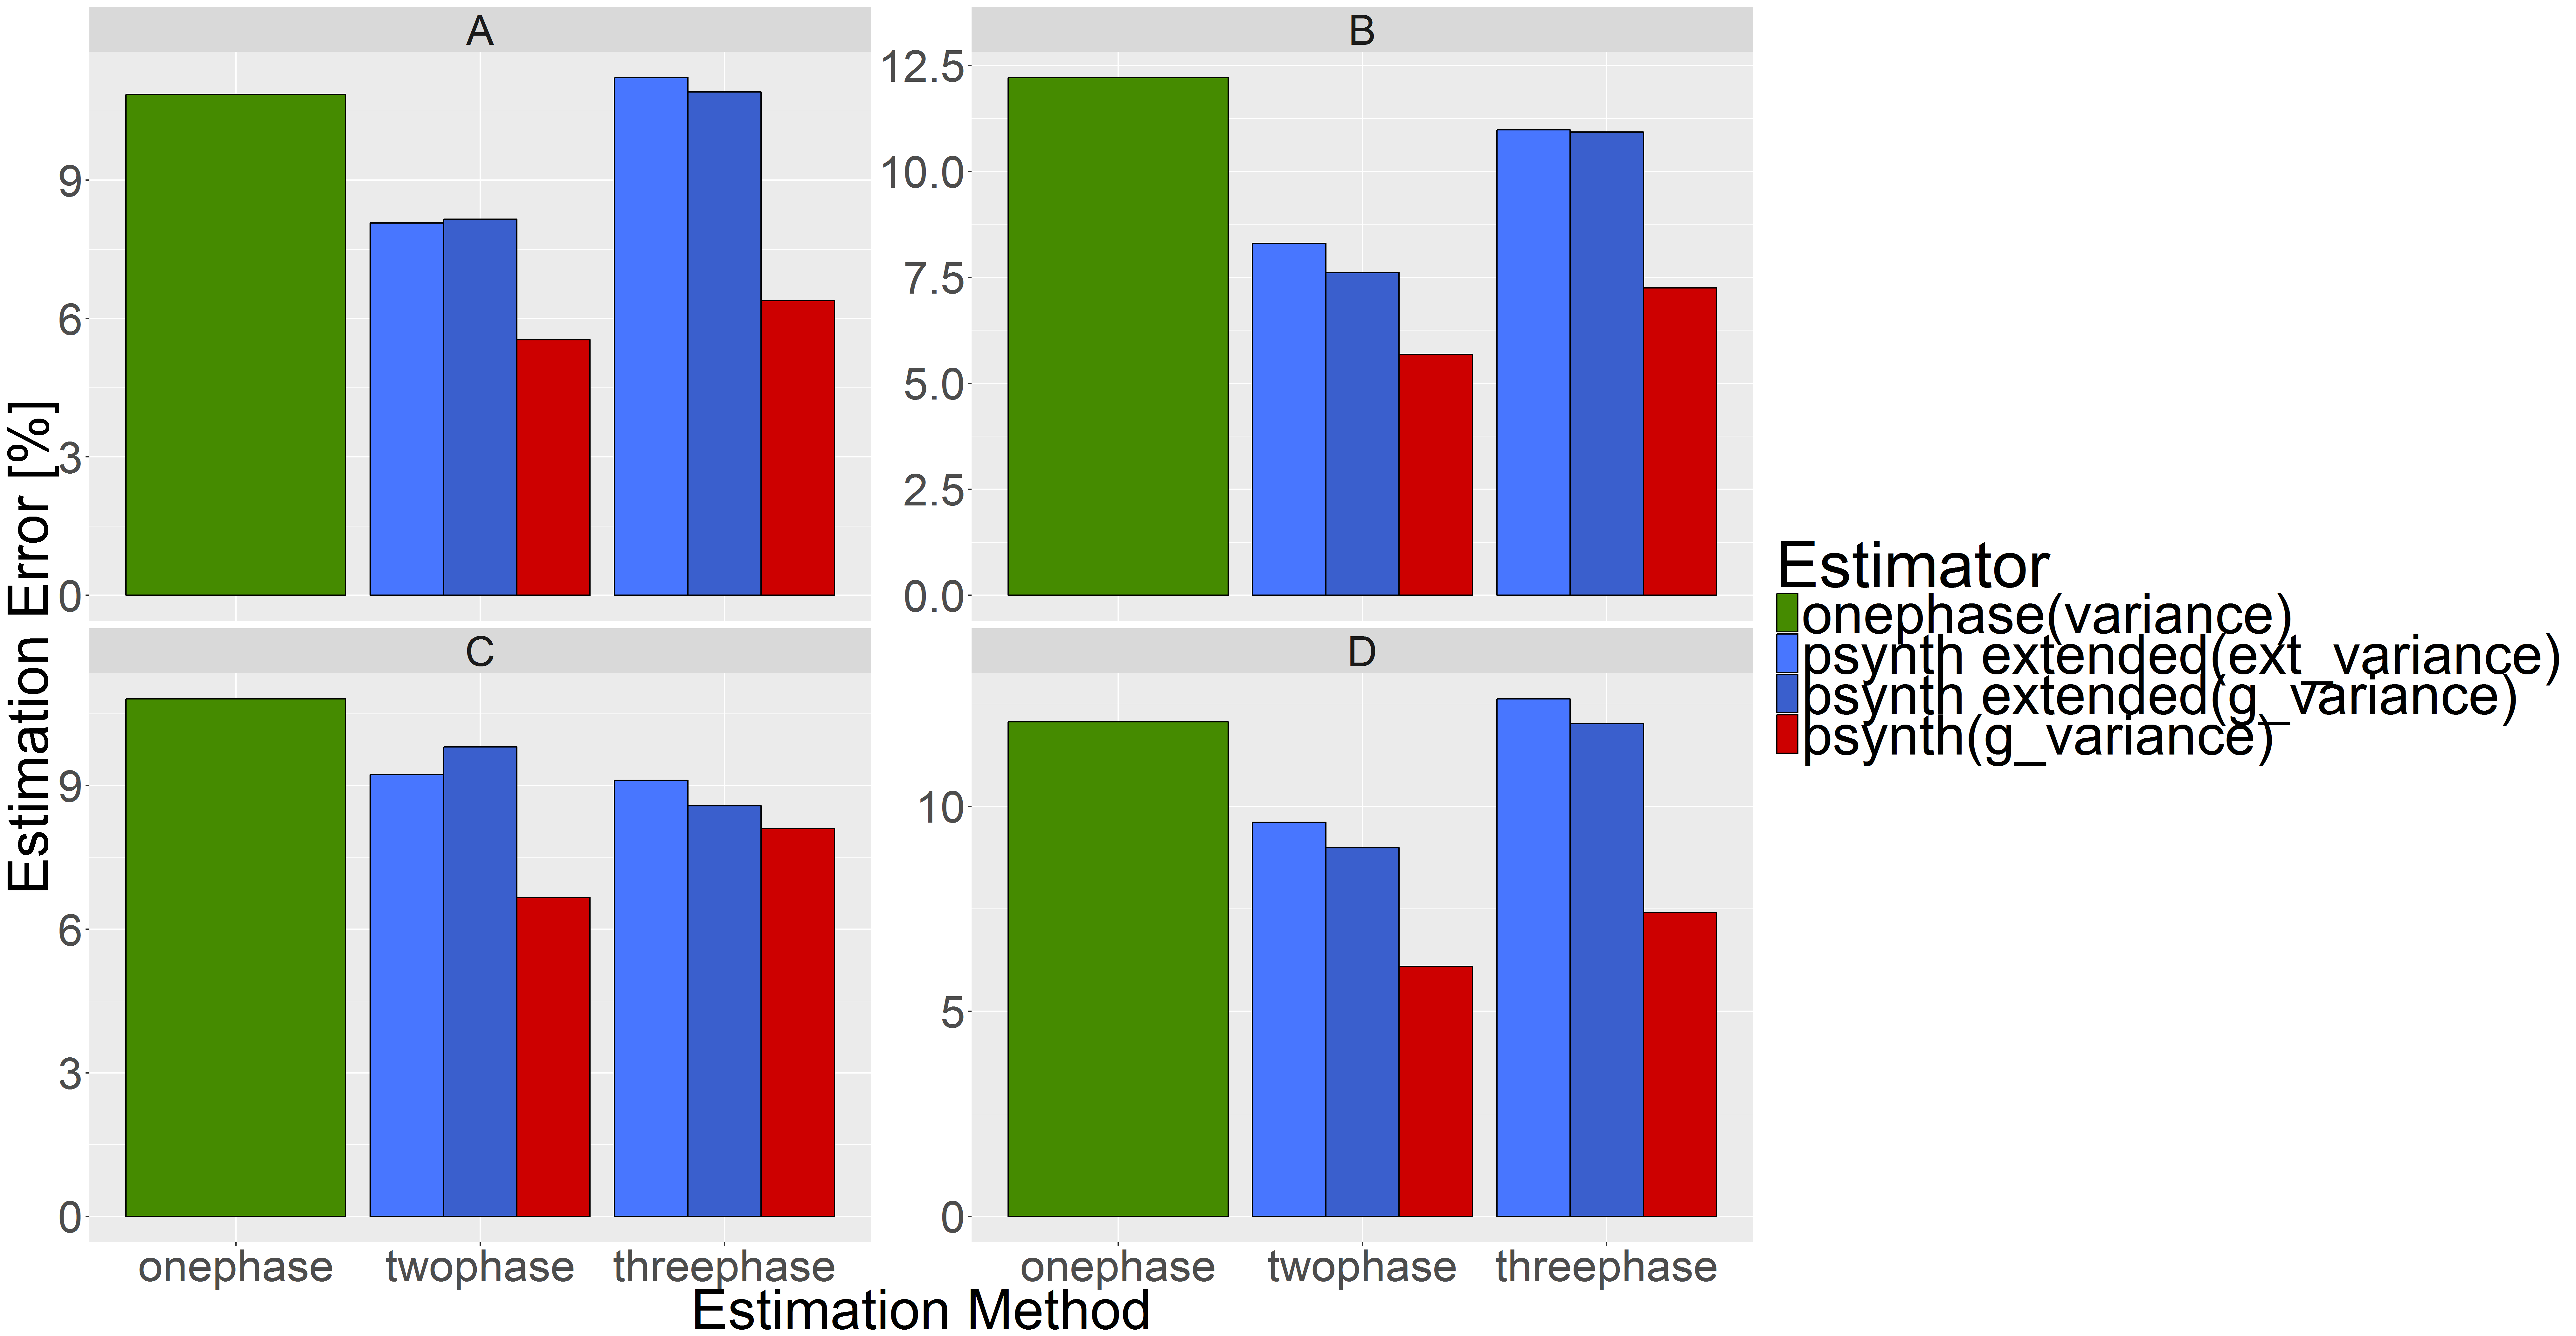
\includegraphics{Grafiken/Jstat_article/plot_error.png}}
\end{figure}

\newpage

Whereas the estimation errors are plotted by default, the point estimates and confidence intervals are returned when setting the argument \code{yvar = "estimate"}. Note that the graphics can arbitrarily be extended by additional \pkg{ggplot2} parameterizations.

\begin{small}
\begin{Schunk}
\begin{Sinput}
R> plot(grisons.sae.table, ncol = 2, yvar = "estimate") +
+    ylab("Timber Volume [m3/ha]")
\end{Sinput}
\end{Schunk}
\end{small}

\begin{figure}[h]
\centering
\resizebox{0.85\hsize}{!}{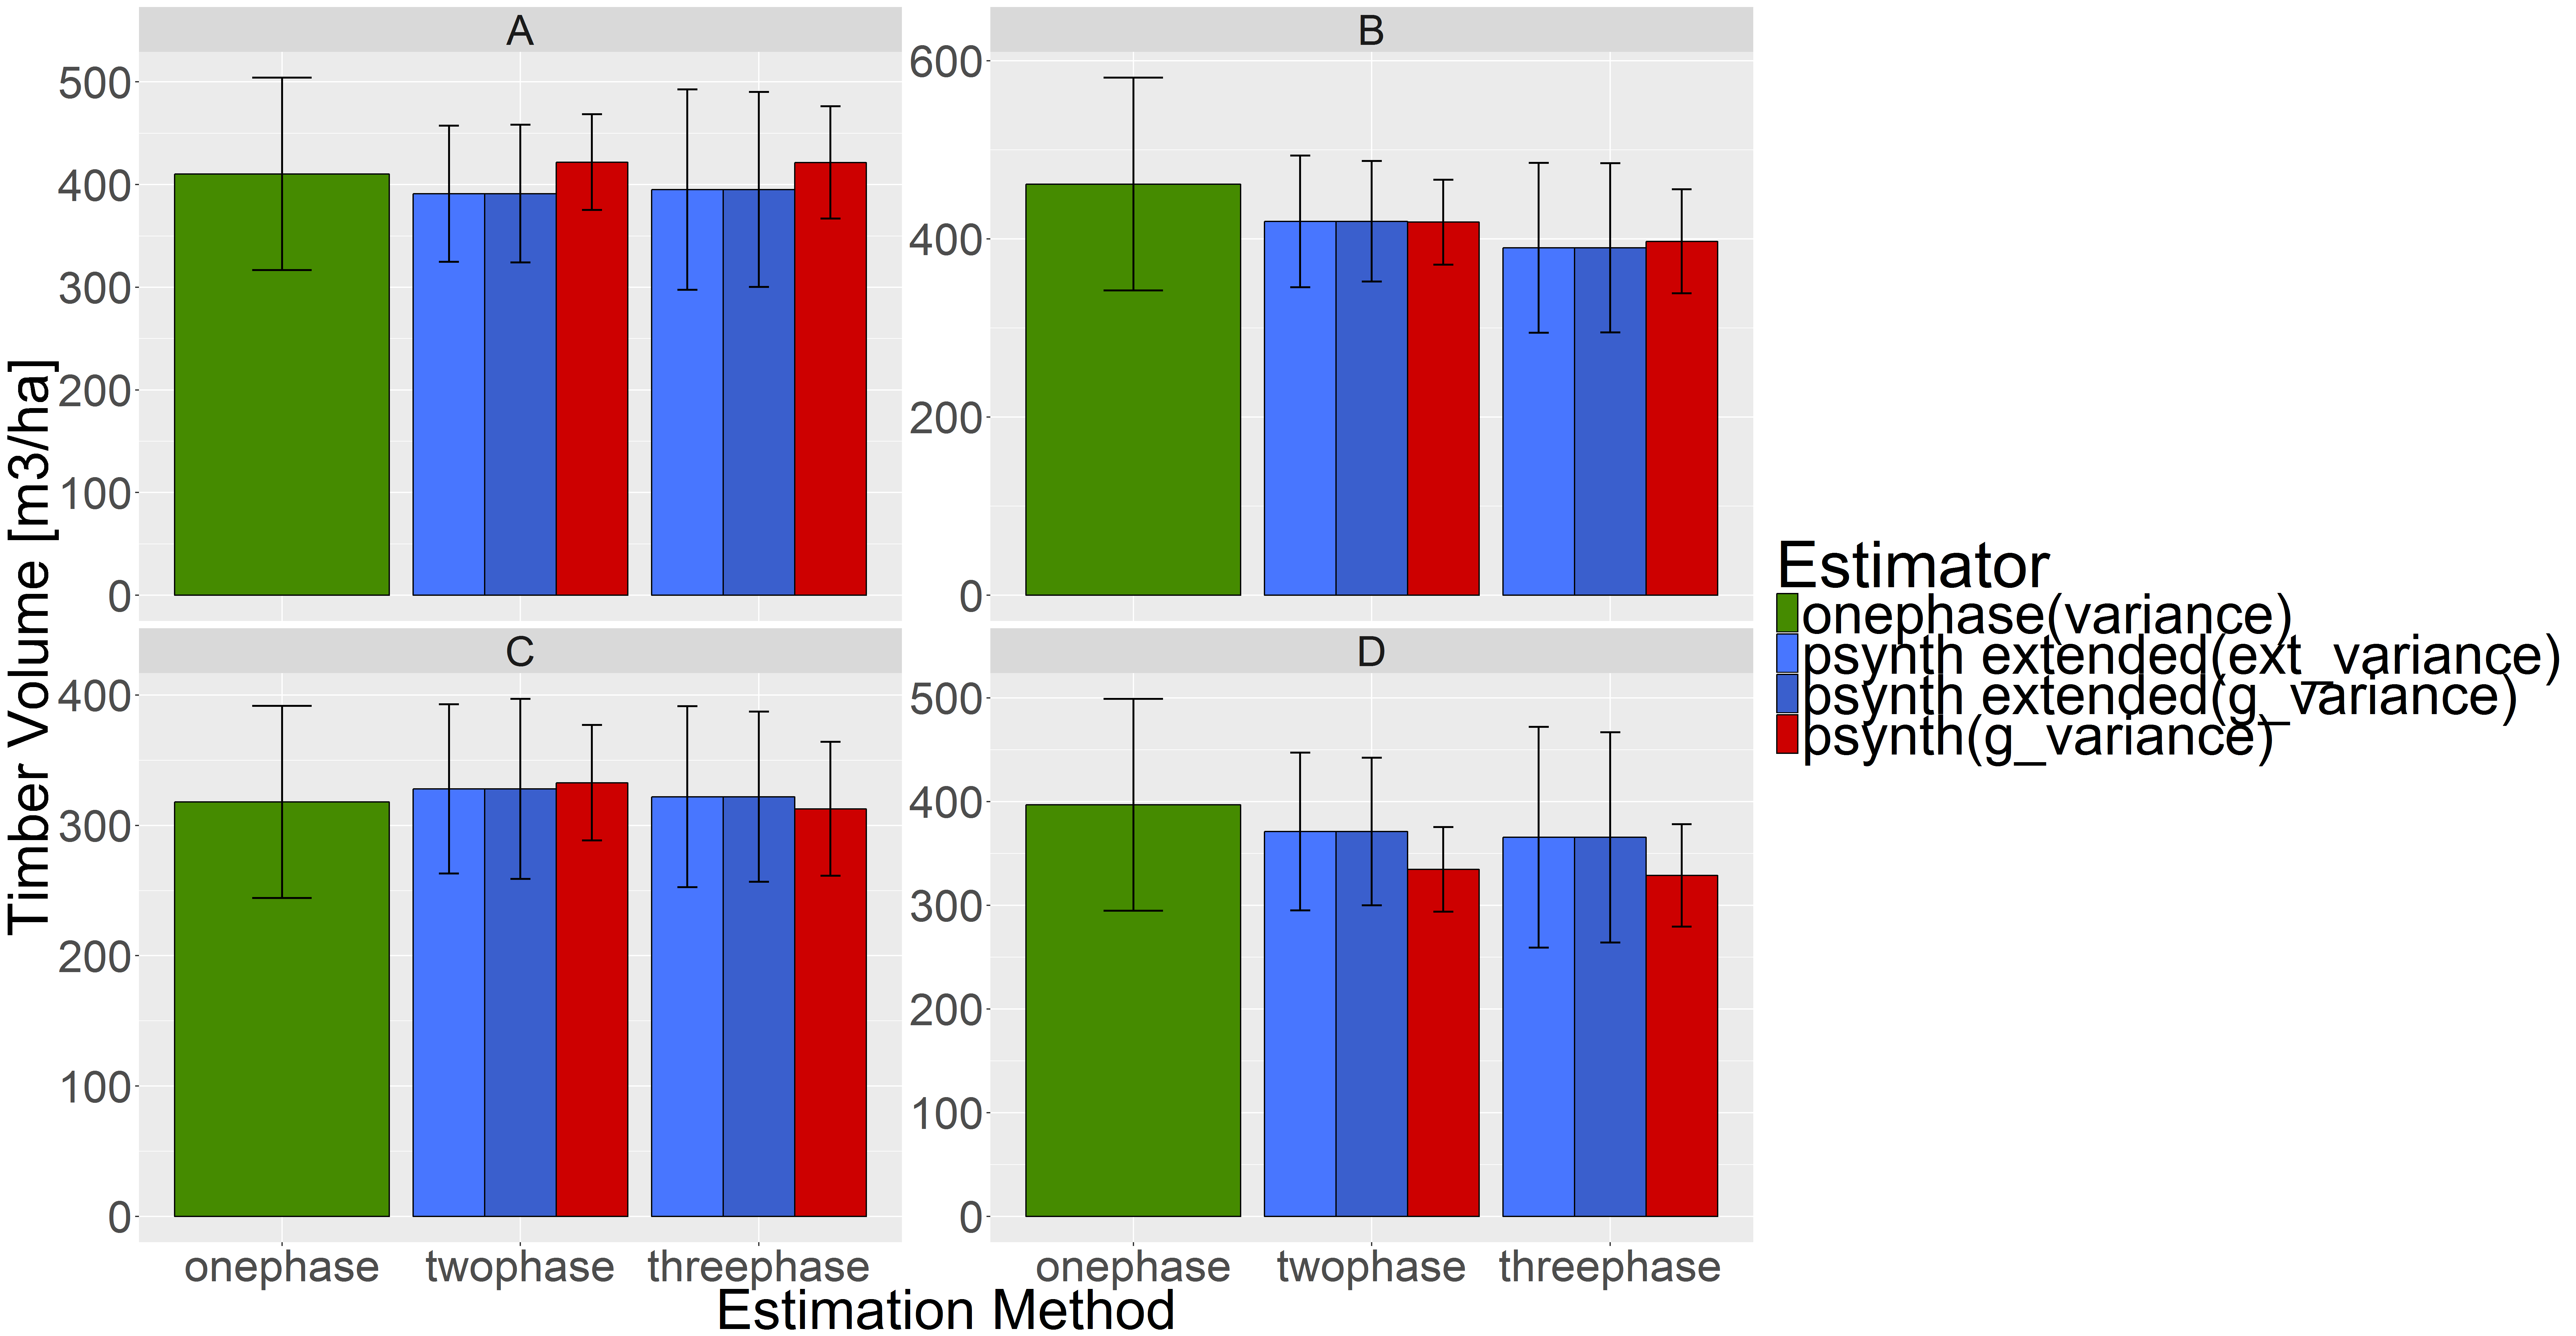
\includegraphics{Grafiken/Jstat_article/plot_est_ci.png}}
\end{figure}


%------------------------------------------------------------------------------------------------%
% ---------------------------------------- Future Plans---- ------------------------------------ %

\section{Future plans}
\label{sec:future}

The \pkg{forestinventory} package currently provides a fairly well-rounded toolkit for forestry inventorists to integrate auxiliary information into their estimates using the model-assisted methods under the design-based approach.  Although 32 combinations of inventory scenarios, estimators and sample designs are covered, there are still potential improvements planned for the future. As this is an open-source project, everyone is encouraged to give feedback and/or make contributions to the package's development page on GitHub \citep{github_forestinventory}. Currently planned extensions include:

\begin{itemize}
\item Implement parallel procedures for efficiently calculating many small areas.
\item Allow functions to accept objects of class \code{data.table} from the \pkg{data.table} package \citep{dt2017} to improve memory efficiency.
\item Enable the user to choose other types of models than linear regressions fitted with OLS.
\end{itemize}

%------------------------------------------------------------------------------------------------%
% ---------------------------------------- Acknowledgements ------------------------------------ %

\section*{Acknowledgements}

We want to express our gratitude to Prof. H. Heinimann (Chair of Land Use Engineering, ETH Zurich) for supporting this study and providing the possibility of working on the package. We also want to thank Daniel Mandallaz for his support in completing the range of the already published estimators in the frame of the three-phase small area estimators, as well as many helpful discussions and advice throughout the implementation of our package. Our thanks also go to Meinrad Abegg for proofreading the manuscript, and to the Amt f{\"u}r Wald und Naturgefahren of the Swiss canton of grisons for providing the example data.

